\documentclass{bredelebeamer}

\renewcommand<>{\item}{\beameroriginal\item\vspace{\stretch{.1}}}
\usefonttheme{professionalfonts} % using non standard fonts for beamer
\usefonttheme{serif} % default family is serif
\usepackage[T1]{fontenc}
\usepackage{lmodern}
\usepackage[]{media9}
\setbeamertemplate{itemize/enumerate body begin}{\Large}
\setbeamertemplate{itemize/enumerate subbody begin}{\large}
\setbeamertemplate{itemize/enumerate subsubbody begin}{\large}

\setbeamertemplate{enumerate item}{%
  \usebeamercolor[bg]{item projected}%
  \raisebox{1.5pt}{\colorbox{bg}{\color{fg}\footnotesize\insertenumlabel}}%
}

%%%%%%%%%%%%%%%%%%%%%%%%%%%%%%%%%%%%%%%%%%%%%%%%

\title[Exit Seminar]{\huge Visualizing RNA-seq data: Pertinence, software, and applications}

\author[Lindsay Rutter (ISU)]{\Large Exit Seminar\\ Lindsay Rutter\\ \vspace{9mm} \normalsize \textbf{Program of Study Committee:}\\ Dianne Cook (Major Professor)\\ Amy Toth (Major Professor)\\ Heike Hofmann\\ Daniel Nettleton\\ James Reecy}


\date[May 1, 2018]{\small May 1, 2018}


%%%%%%%%%%%%%%%%%%%%%%%%%%%%%%%%%%%%%%%%%%%%%%%%%%%%%%%%%%%%%%%%%%%%%
\begin{document}

\shorthandoff{:}

\begin{frame}
  \titlepage
\end{frame}

\begin{frame}{Chapter Outline}

\begin{itemize}
		\item \textbf{Chapter 1}\\ 
		Visualization methods for genealogical datasets

		\item \textbf{Chapter 2}\\  
		The case for visualization methods in RNA-seq data analysis

		\item \textbf{Chapter 3}\\
		Software for visualization methods in RNA-seq data analysis
		
		\item \textbf{Chapter 4}\\  
		RNA-seq analysis of diet quality and viral infection in \textit{Apis mellifera}

	\end{itemize}
\end{frame}

%%%%%%%%%%%%%%%%%%%%%%%%%%%%%%%%% CHAPTER 1 %%%%%%%%%%%%%%%%%%%%%%%%%%%%%
\section{Visualizing genealogy}

\begin{frame}[noframenumbering]
\begin{center}
\fcolorbox{black}{titleColor}{
\begin{minipage}{\textwidth}
\begin{center}
\huge \textbf{Chapter 1:} Visualization methods for\\
genealogical datasets
\end{center}
\end{minipage}
}
\end{center}
\end{frame}

\begin{frame}{}
\begin{figure}
\centering
\fbox{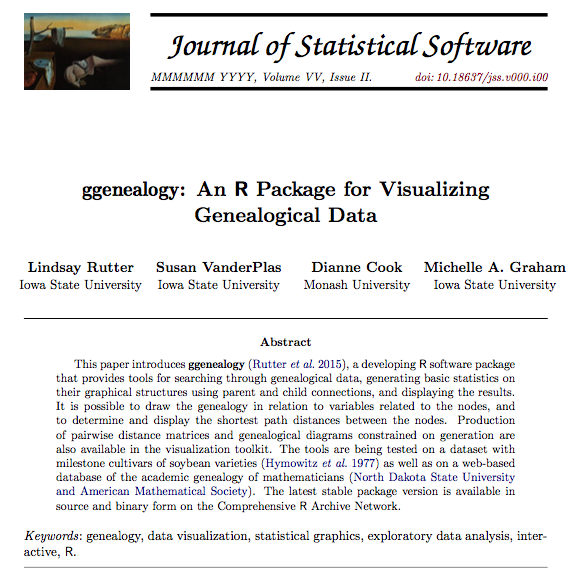
\includegraphics[scale=0.37]{images/JSS.png}}
\end{figure}
\end{frame}

\begin{frame}{}
\begin{figure}
\centering
\fbox{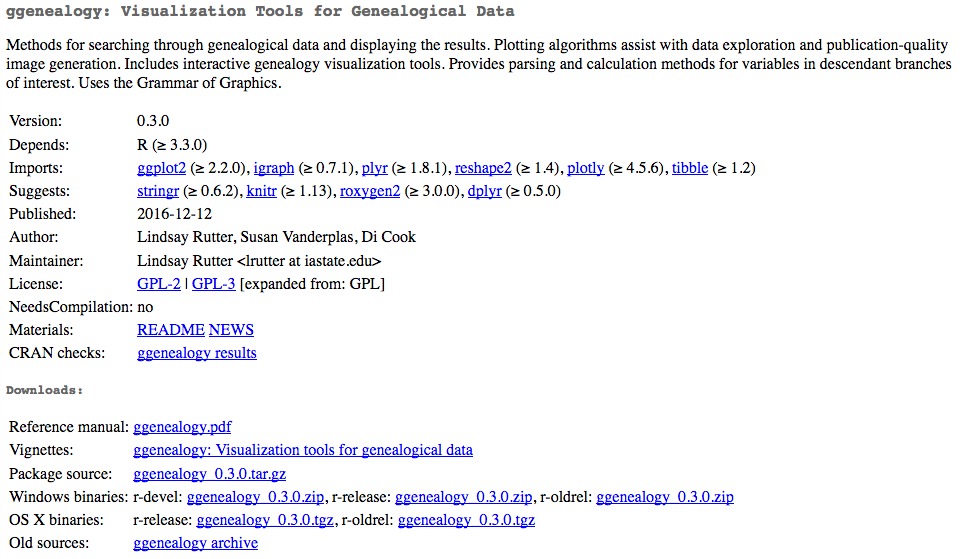
\includegraphics[scale=0.3]{images/ggenealogyCRAN.png}}
\end{figure}
\end{frame}

%%%%%%%%%%%%%%%%%%%%%%%%%%%%%%%%% CHAPTER 2 %%%%%%%%%%%%%%%%%%%%%%%%%%%%%
\section{Why visualize RNA-seq}

\begin{frame}[noframenumbering]
\begin{center}
\fcolorbox{black}{titleColor}{
\begin{minipage}{\textwidth}
\begin{center}
\huge \textbf{Chapter 2:} The case for visualization \\
methods in RNA-seq analysis
\end{center}
\end{minipage}
}
\end{center}
\end{frame}

\begin{frame}
\begin{figure}
\centering
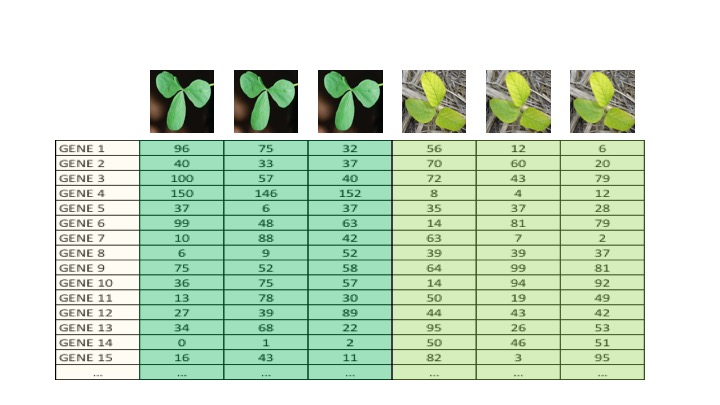
\includegraphics[scale=0.47]{images/rnaseq1.jpg}
\end{figure}
\end{frame}

\begin{frame}[noframenumbering]
\begin{figure}
\centering
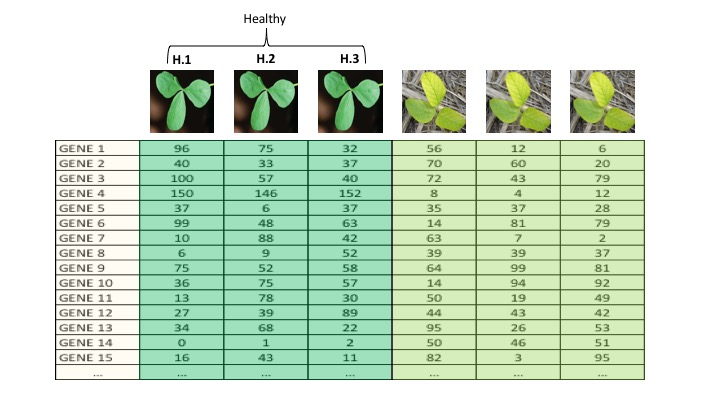
\includegraphics[scale=0.47]{images/rnaseq2.jpg}
\end{figure}
\end{frame}

\begin{frame}[noframenumbering]
\begin{figure}
\centering
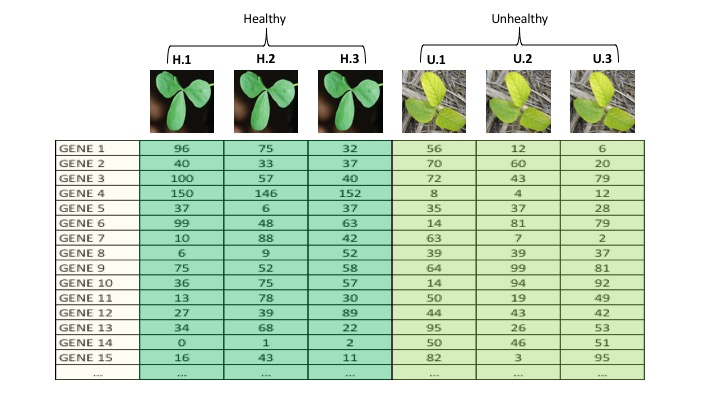
\includegraphics[scale=0.47]{images/rnaseq3.jpg}
\end{figure}
\end{frame}

\begin{frame}[noframenumbering]
\begin{figure}
\centering
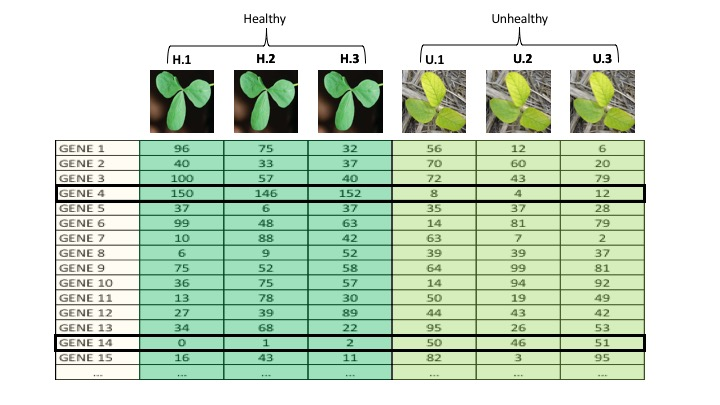
\includegraphics[scale=0.47]{images/rnaseq4.jpg}
\end{figure}
\end{frame}

\begin{frame}[noframenumbering]
\begin{figure}
\centering
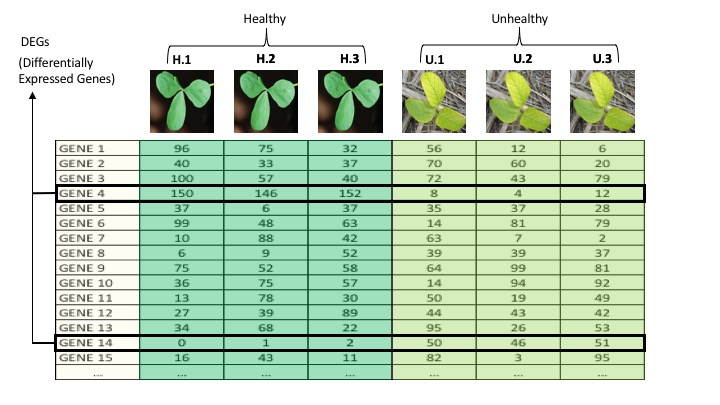
\includegraphics[scale=0.47]{images/rnaseq5.jpg}
\end{figure}
\end{frame}

\begin{frame}{}
\begin{figure}
\centering
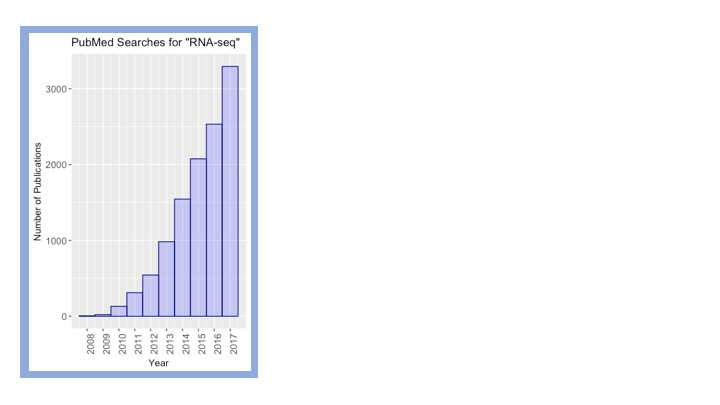
\includegraphics[scale=0.53]{images/pubMedNorm1.jpg}
\end{figure}
\end{frame}

\begin{frame}[noframenumbering]
\begin{figure}
\centering
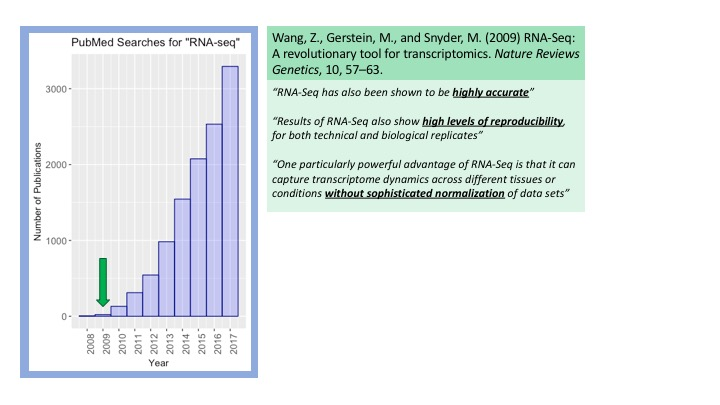
\includegraphics[scale=0.53]{images/pubMedNorm2.jpg}
\end{figure}
\end{frame}

\begin{frame}[noframenumbering]
\begin{figure}
\centering
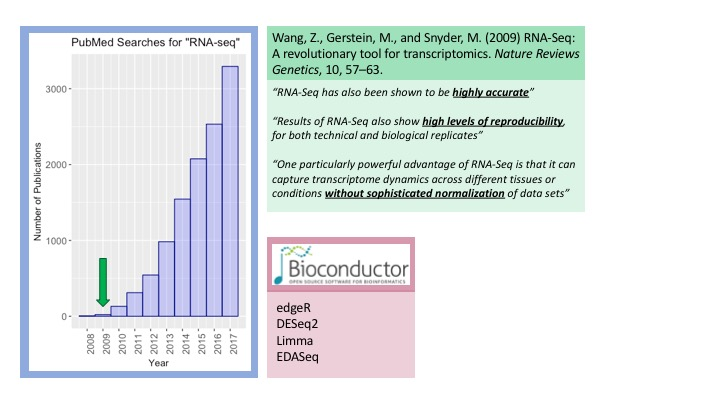
\includegraphics[scale=0.53]{images/pubMedNorm3.jpg}
\end{figure}
\end{frame}

\begin{frame}{}
\begin{figure}
\centering
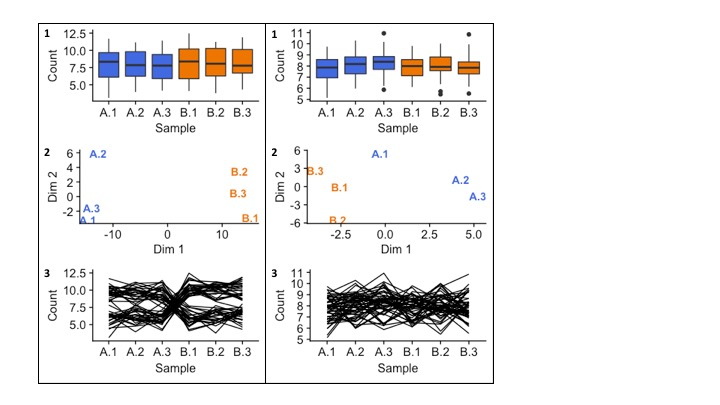
\includegraphics[scale=0.58]{images/mdsBox1.jpg}
\end{figure}
\end{frame}

\begin{frame}[noframenumbering]
\begin{figure}
\centering
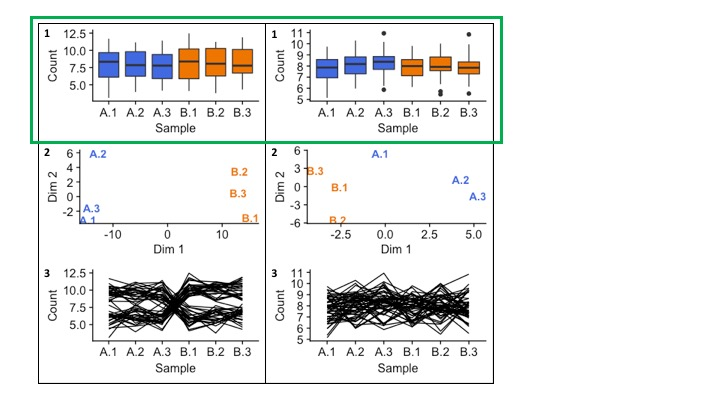
\includegraphics[scale=0.58]{images/mdsBox2.jpg}
\end{figure}
\end{frame}

\begin{frame}[noframenumbering]
\begin{figure}
\centering
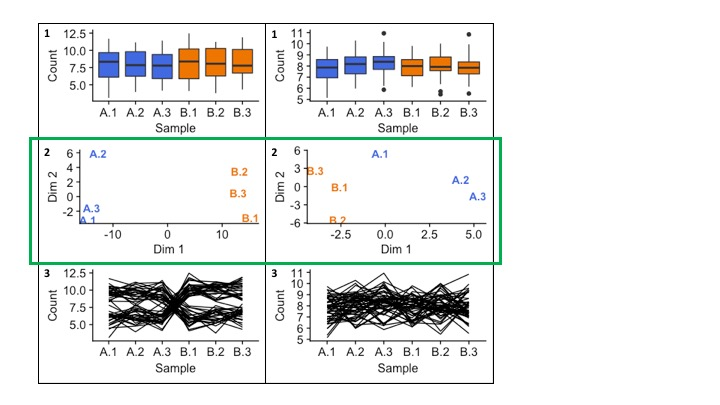
\includegraphics[scale=0.58]{images/mdsBox3.jpg}
\end{figure}
\end{frame}

\begin{frame}[noframenumbering]
\begin{figure}
\centering
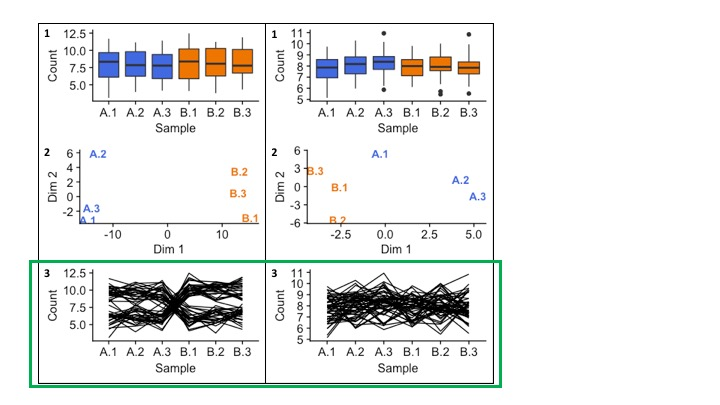
\includegraphics[scale=0.58]{images/mdsBox4.jpg}
\end{figure}
\end{frame}

\begin{frame}[noframenumbering]
\begin{figure}
\centering
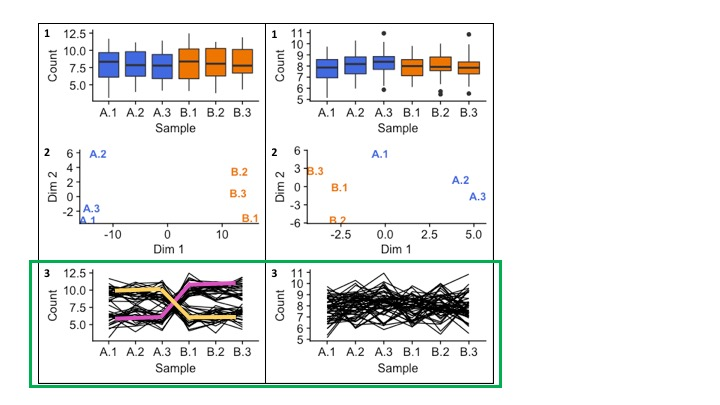
\includegraphics[scale=0.58]{images/mdsBox5.jpg}
\end{figure}
\end{frame}

\begin{frame}{}
\begin{figure}
\centering
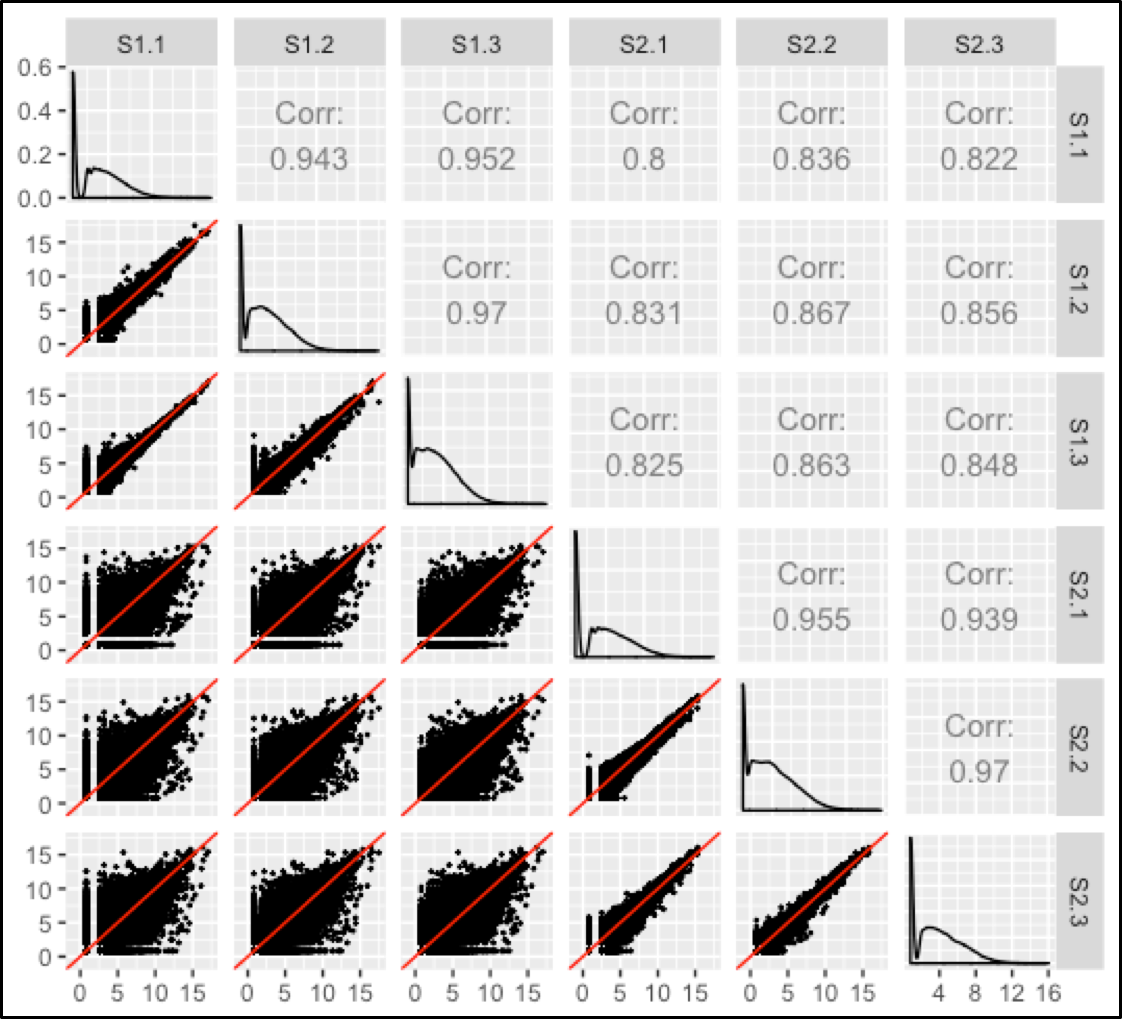
\includegraphics[scale=0.45]{images/sbCNSM1.png}
\end{figure}
\end{frame}

\begin{frame}[noframenumbering]
\begin{figure}
\centering
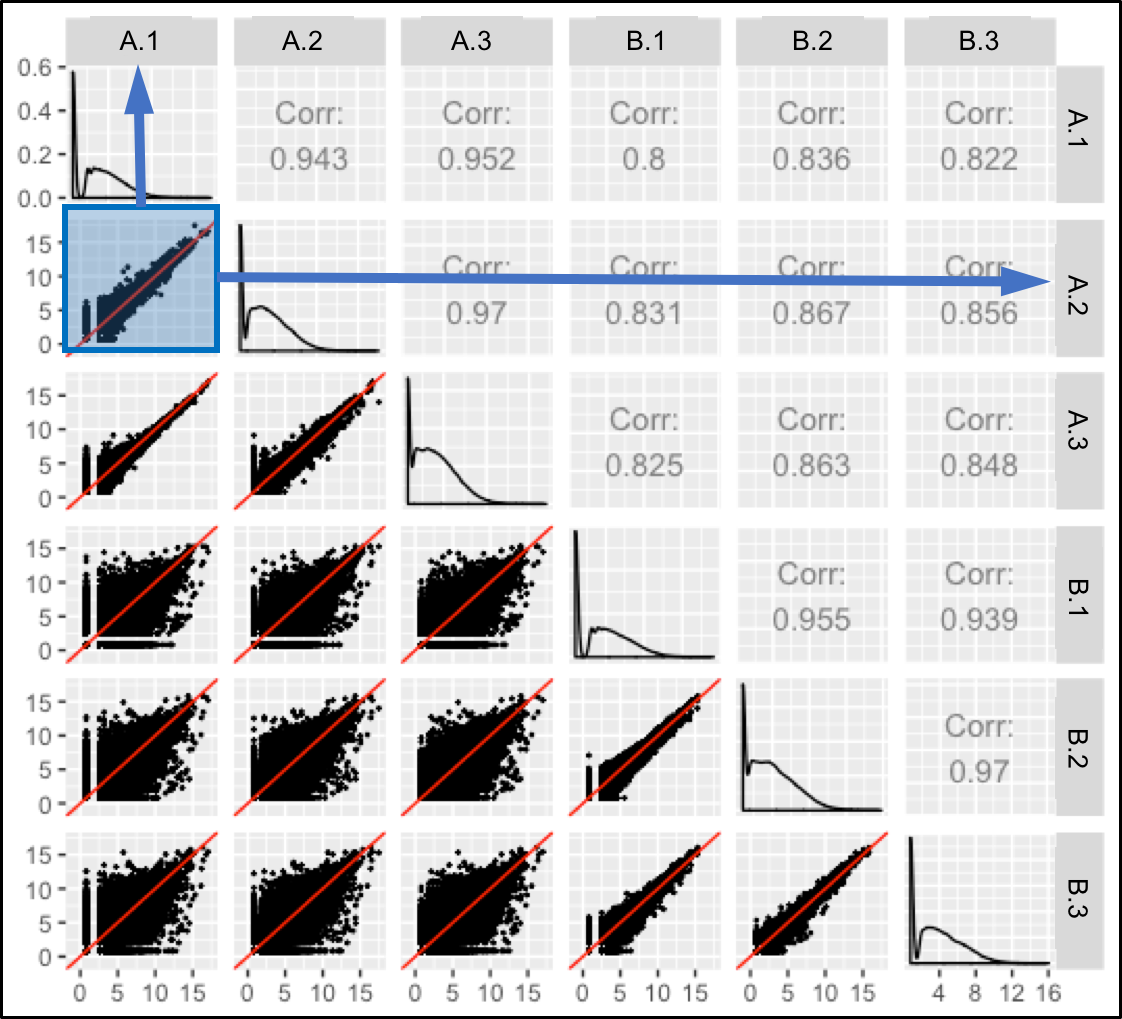
\includegraphics[scale=0.45]{images/sbCNSM2.png}
\end{figure}
\end{frame}

\begin{frame}[noframenumbering]
\begin{figure}
\centering
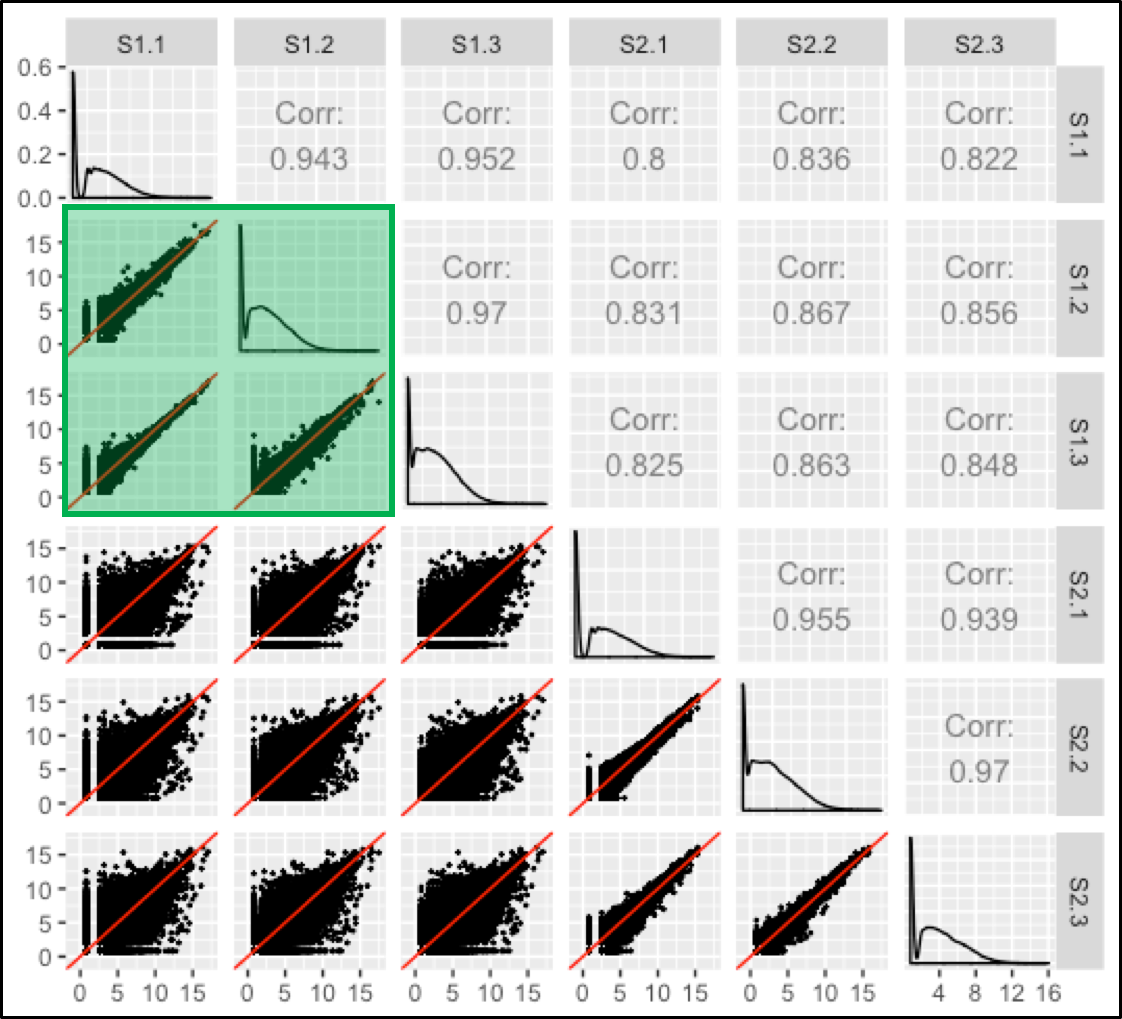
\includegraphics[scale=0.45]{images/sbCNSM3.png}
\end{figure}
\end{frame}

\begin{frame}[noframenumbering]
\begin{figure}
\centering
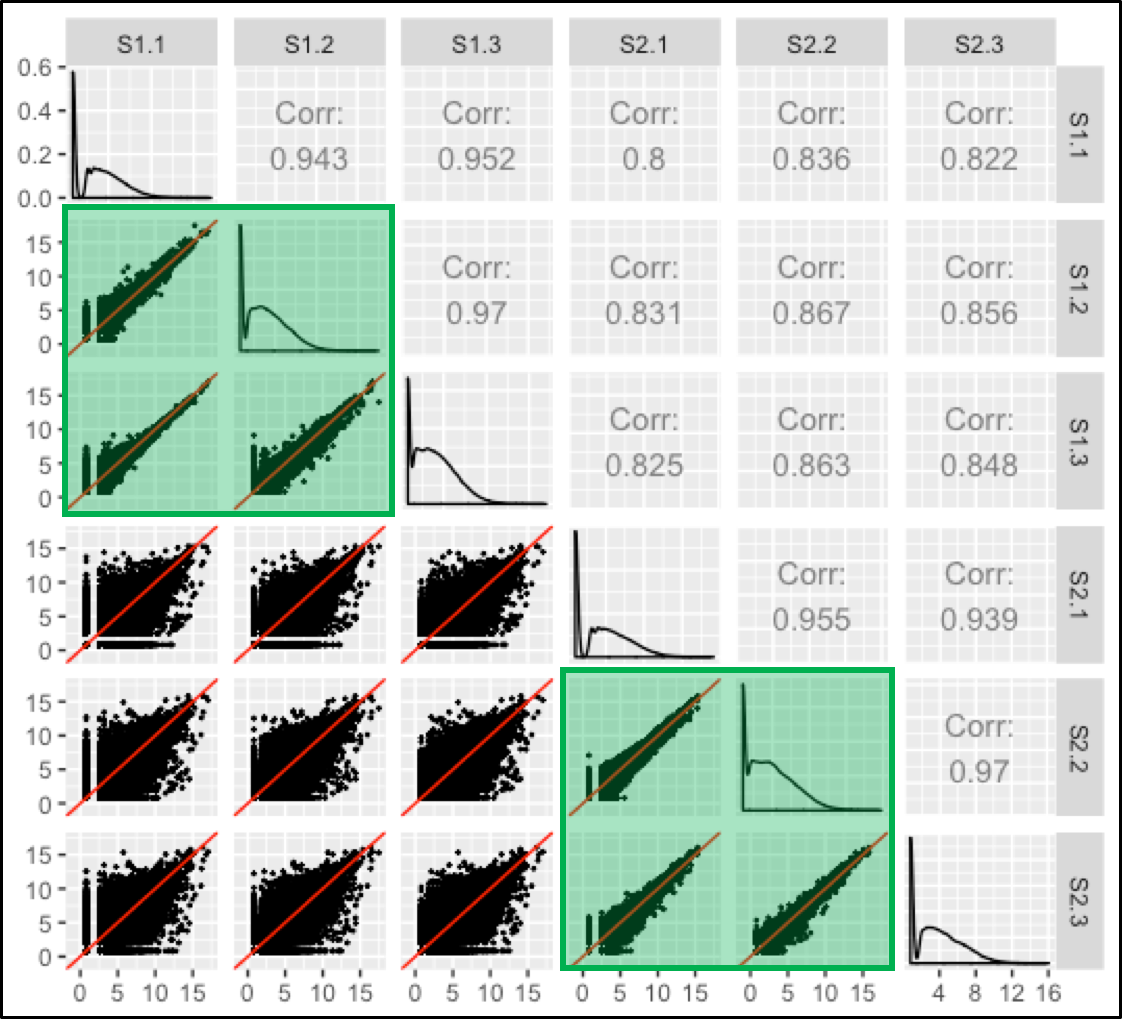
\includegraphics[scale=0.45]{images/sbCNSM4.png}
\end{figure}
\end{frame}

\begin{frame}[noframenumbering]
\begin{figure}
\centering
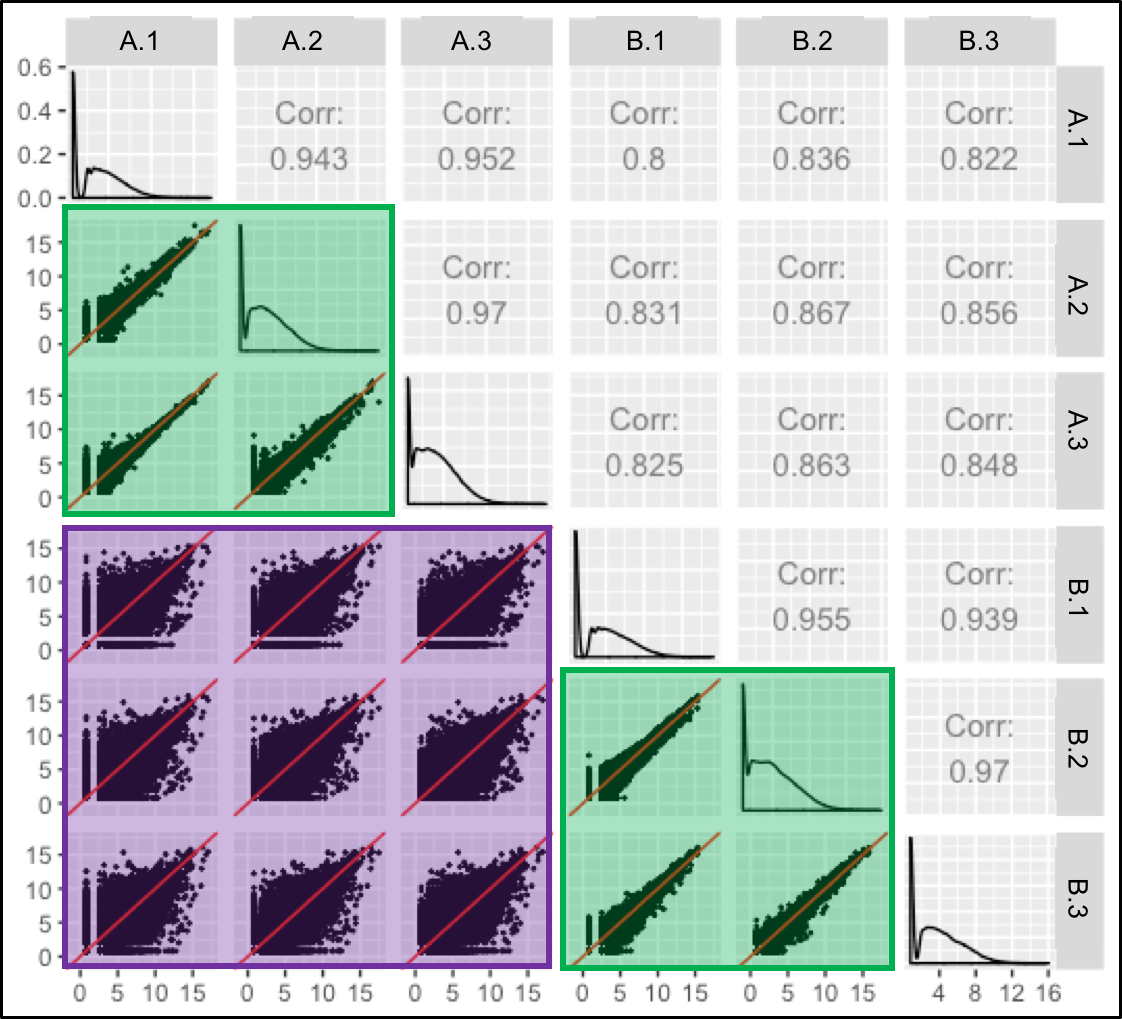
\includegraphics[scale=0.45]{images/sbCNSM5.png}
\end{figure}
\end{frame}







%\centering\href{https://rnaseqvisualization.shinyapps.io/scatmat}{Interactive version}


\begin{frame}{}
\begin{figure}
\centering
\fbox{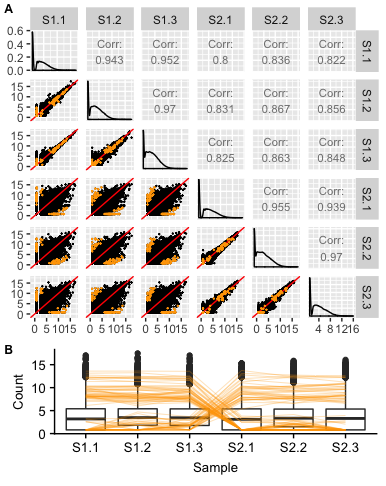
\includegraphics[scale=0.44]{images/sbIRDEG.jpg}}
\end{figure}
\end{frame}

\begin{frame}[noframenumbering]
\begin{figure}
\centering
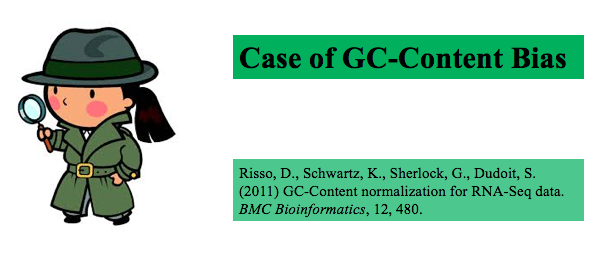
\includegraphics[scale=0.45]{images/case1.png}
\end{figure}
\end{frame}

\begin{frame}{}
\begin{figure}
\centering
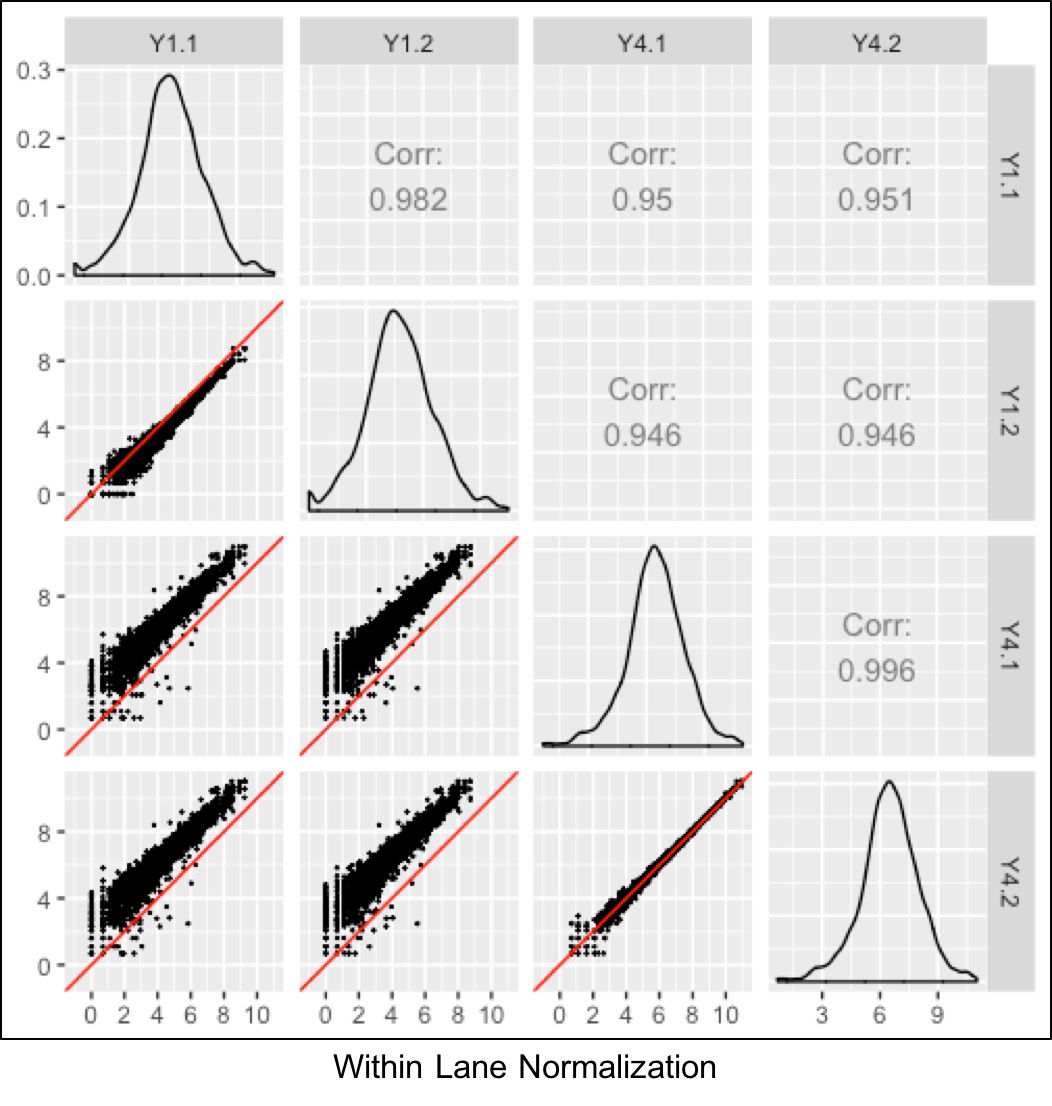
\includegraphics[scale=0.43]{images/yeastWithinBetween.png}
\end{figure}
\end{frame}

\begin{frame}{}
\begin{figure}
\centering
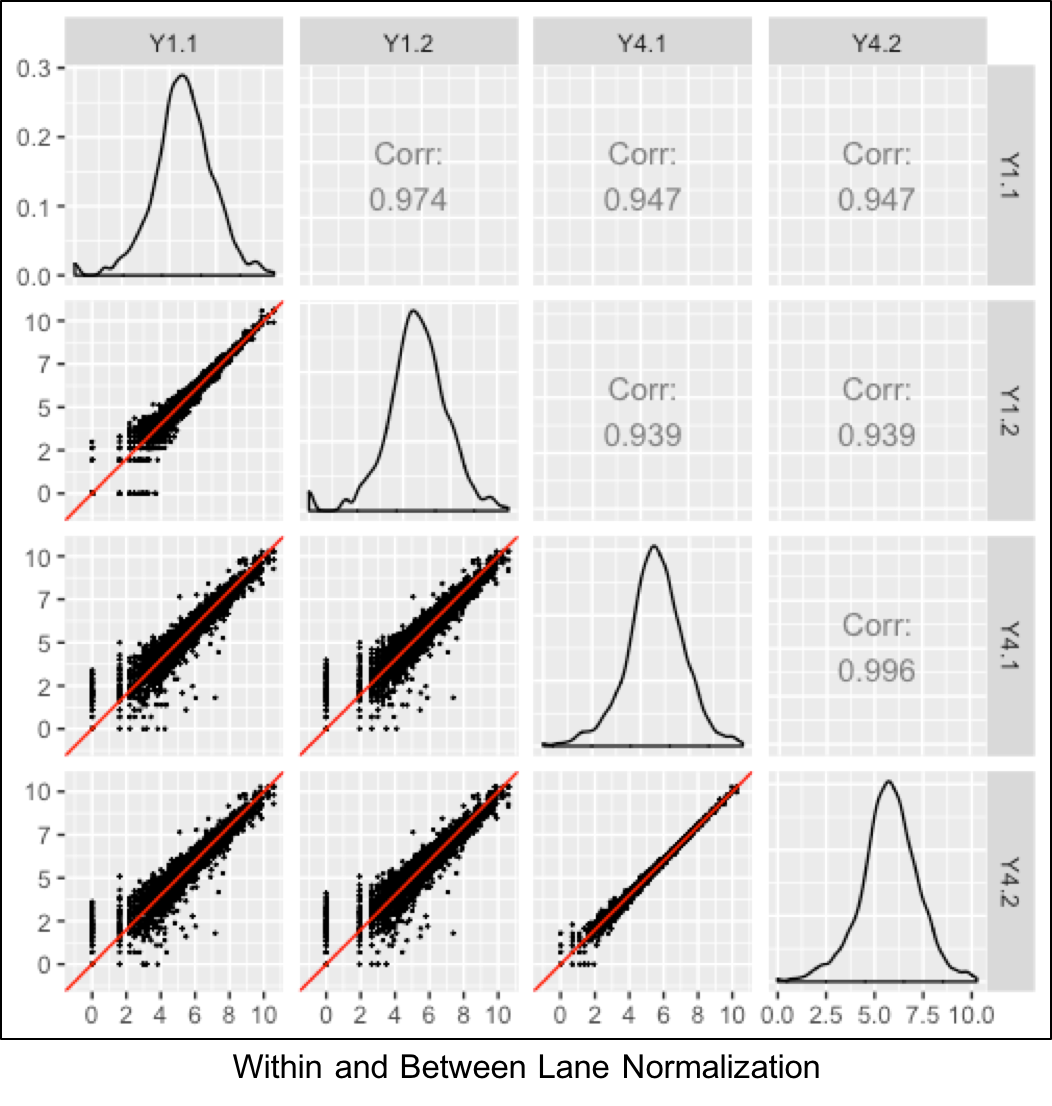
\includegraphics[scale=0.43]{images/yeastWithinBetween2.png}
\end{figure}
\end{frame}

\begin{frame}[noframenumbering]
\begin{figure}
\centering
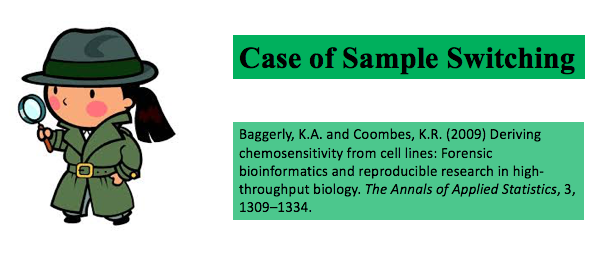
\includegraphics[scale=0.45]{images/case2.png}
\end{figure}
\end{frame}

\begin{frame}{}
\begin{figure}
\centering
\fbox{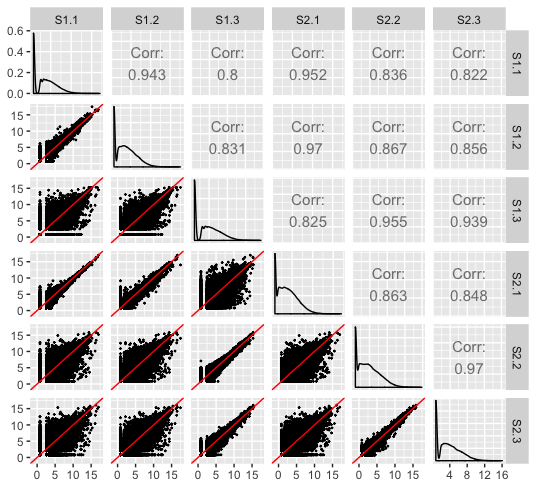
\includegraphics[scale=0.42]{images/sbCNSwitchedSM.jpg}}
\end{figure}
\end{frame}

\begin{frame}[noframenumbering]
\begin{figure}
\centering
\fbox{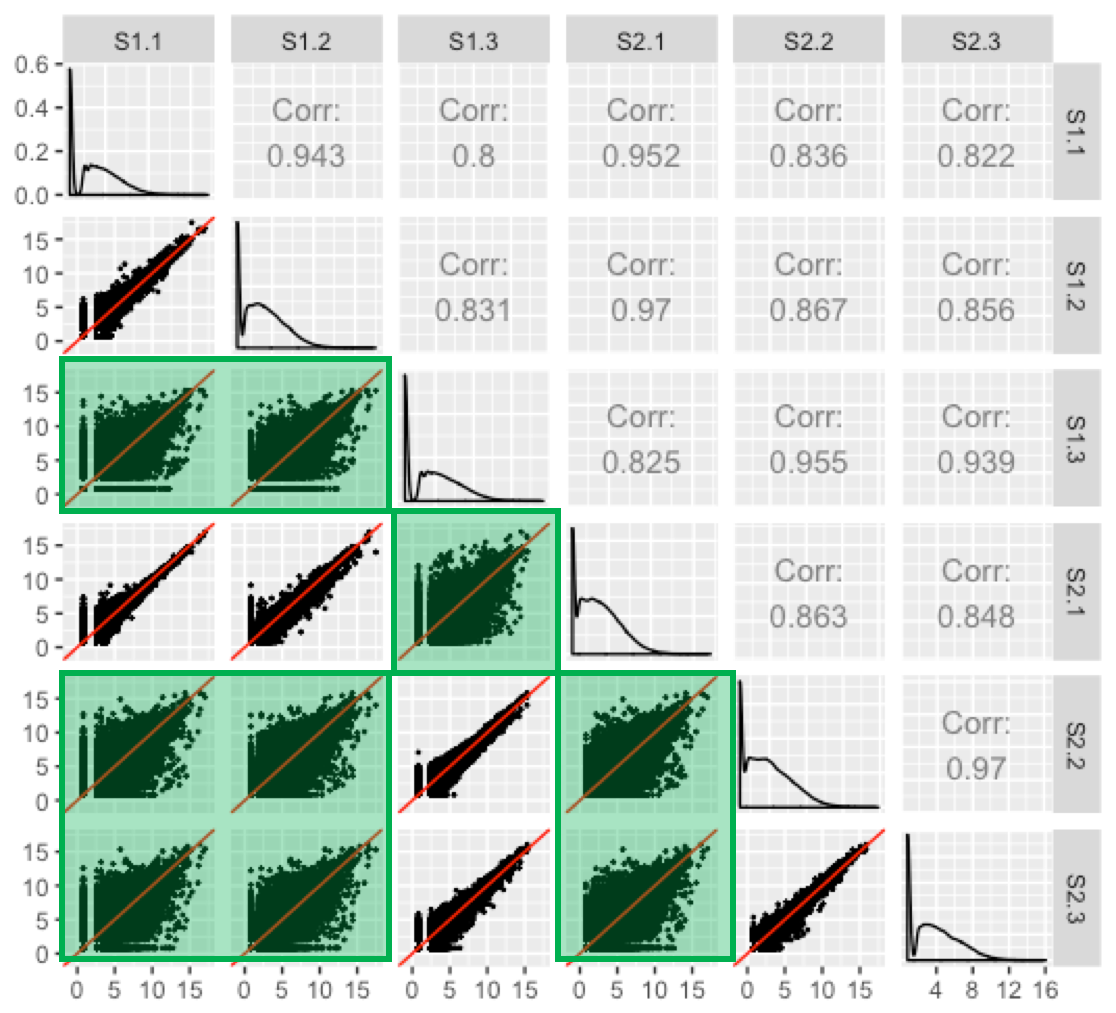
\includegraphics[scale=0.42]{images/sbCNSwitchedSM2.png}}
\end{figure}
\end{frame}

\begin{frame}[noframenumbering]
\begin{figure}
\centering
\fbox{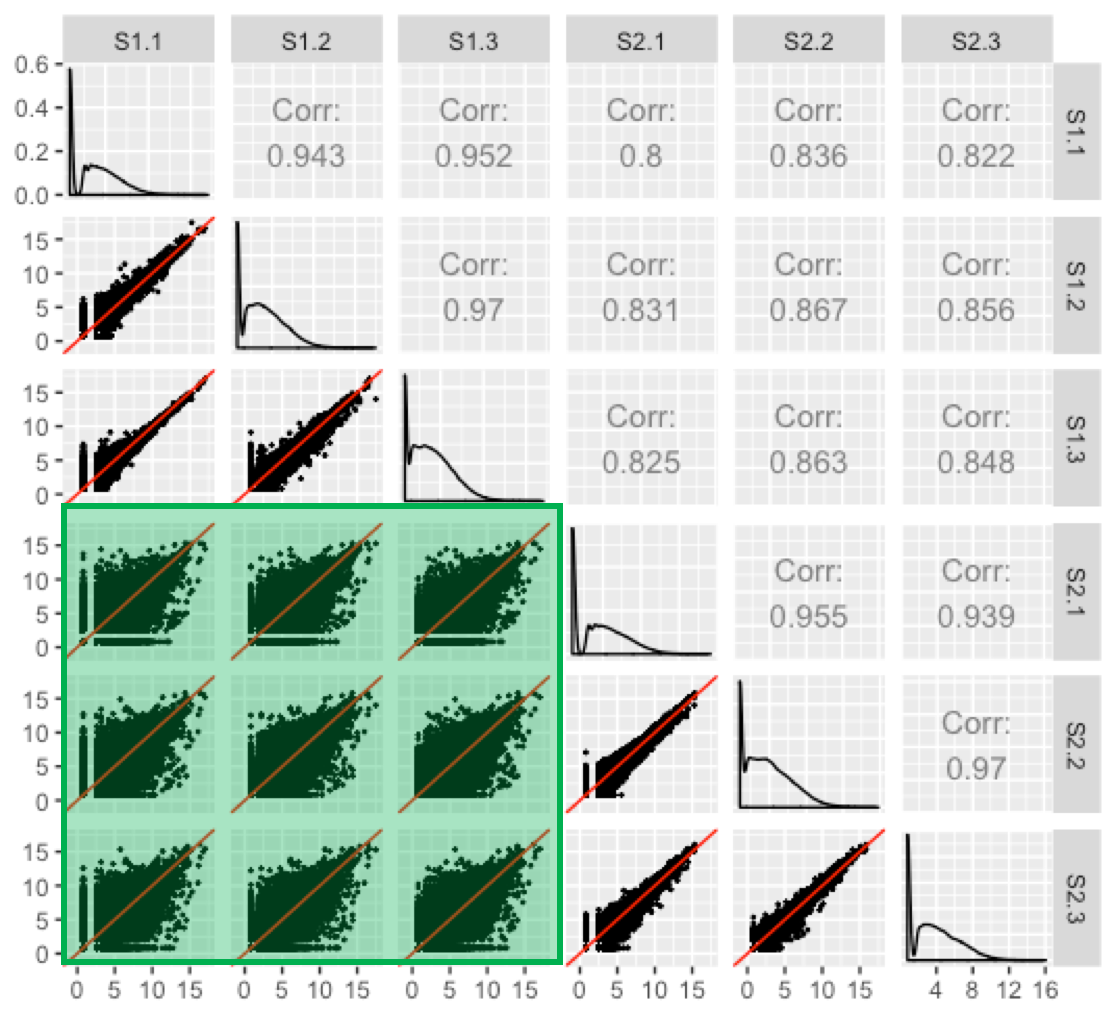
\includegraphics[scale=0.42]{images/sbCNSwitchedSM3.png}}
\end{figure}
\end{frame}

\begin{frame}{}
\begin{figure}
\centering
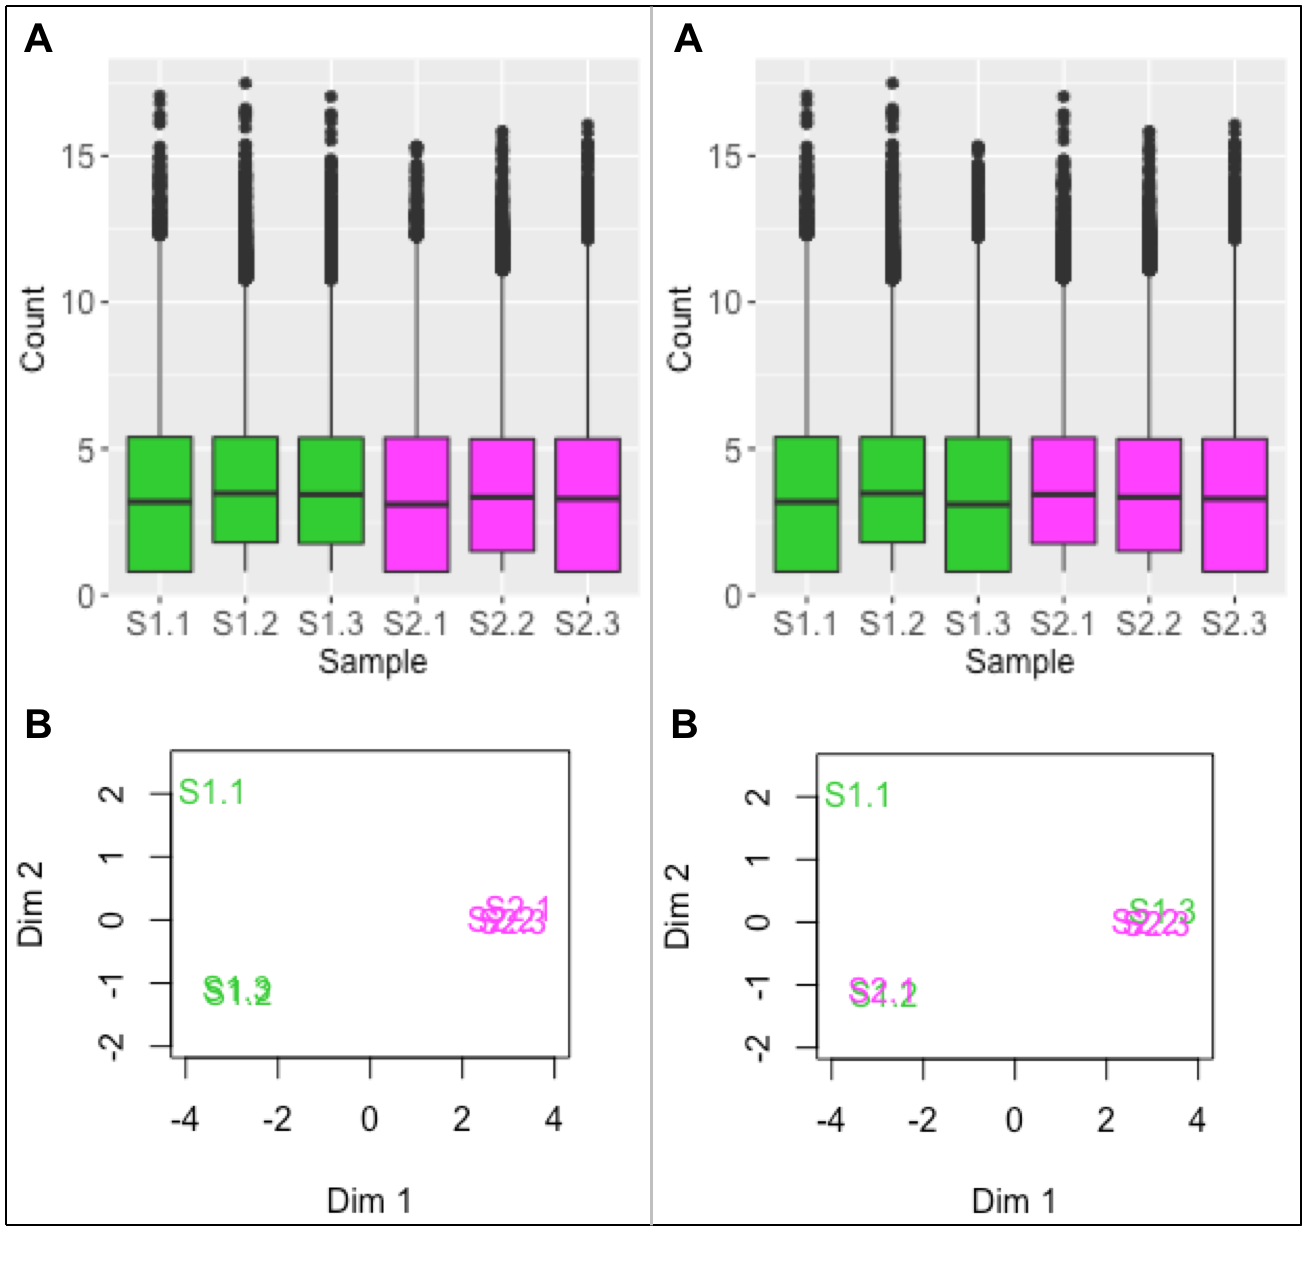
\includegraphics[scale=0.35]{images/mdsSwitch.png}
\end{figure}
\end{frame}

\begin{frame}[noframenumbering]
\begin{figure}
\centering
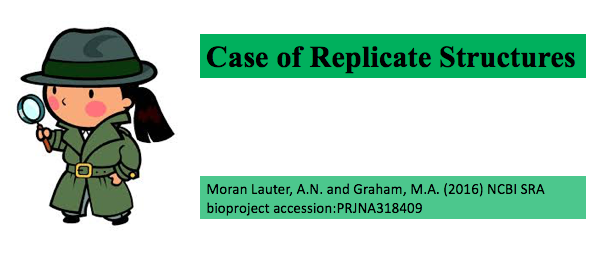
\includegraphics[scale=0.45]{images/case3.png}
\end{figure}
\end{frame}

\begin{frame}{}
\begin{figure}
\centering
\fbox{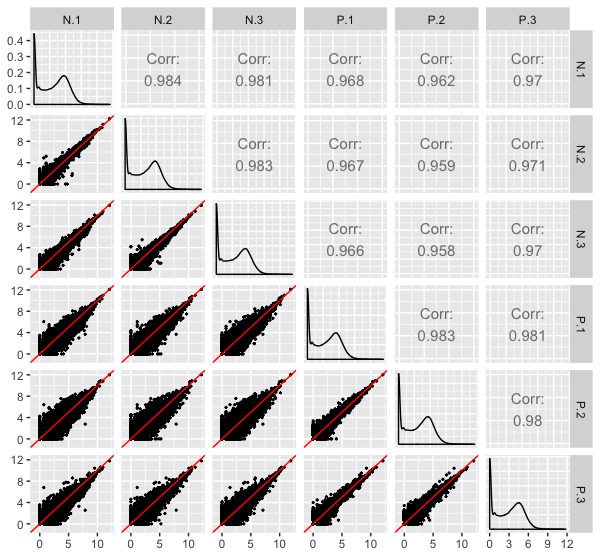
\includegraphics[scale=0.40]{images/sbIRStreak1.png}}
\end{figure}
\end{frame}

\begin{frame}[noframenumbering]
\begin{figure}
\centering
\fbox{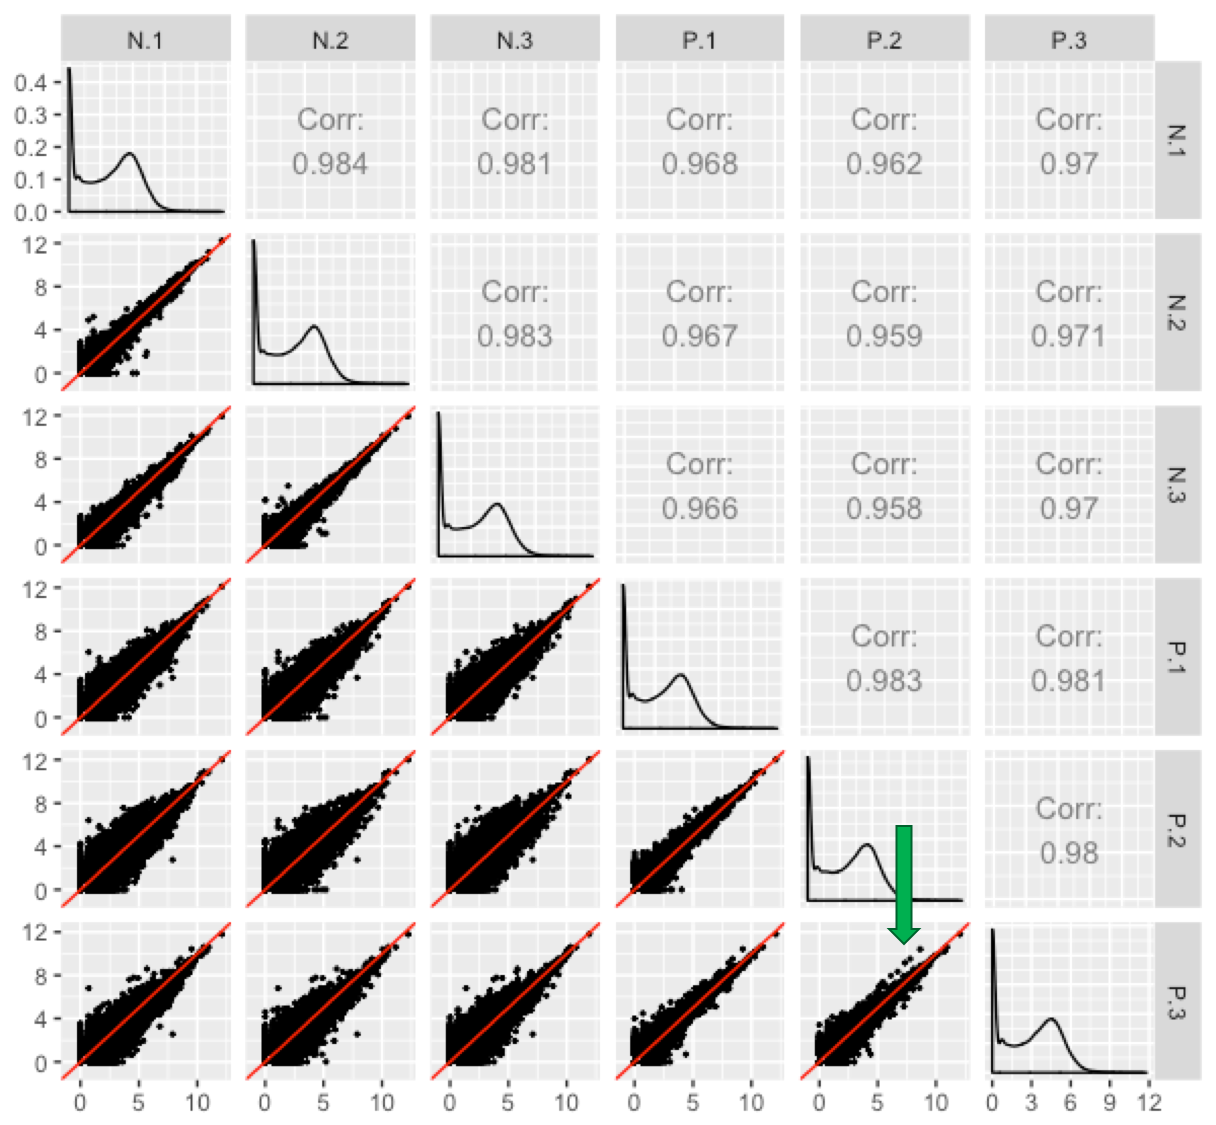
\includegraphics[scale=0.41]{images/sbIRStreak2.png}}
\end{figure}
\end{frame}

\begin{frame}[noframenumbering]
\begin{figure}
\centering
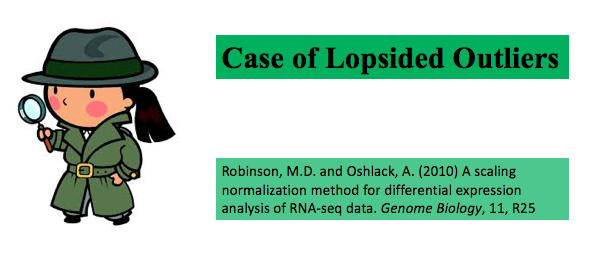
\includegraphics[scale=0.45]{images/case4.png}
\end{figure}
\end{frame}

\begin{frame}{}
\begin{figure}
\centering
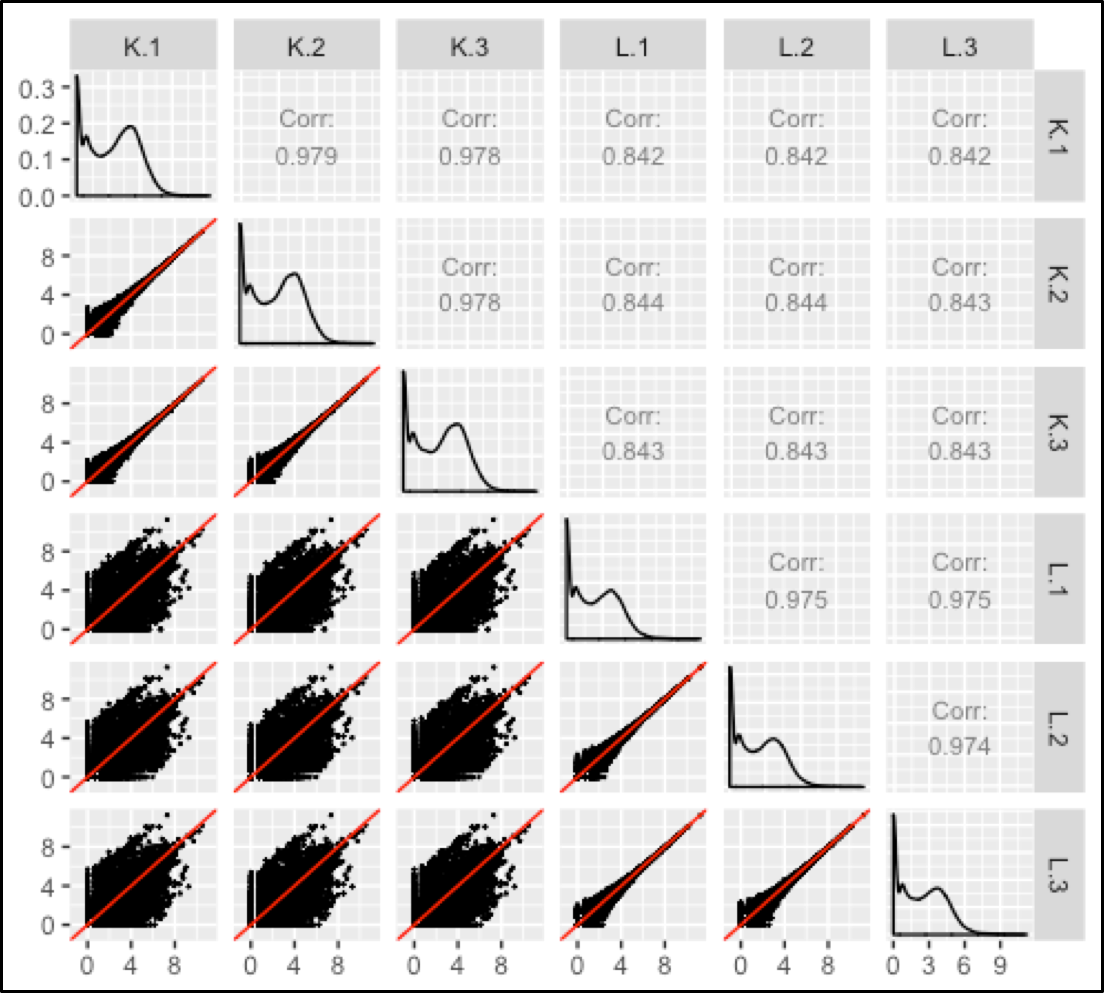
\includegraphics[scale=0.45]{images/lkSM1.png}
\end{figure}
\end{frame}

\begin{frame}[noframenumbering]
\begin{figure}
\centering
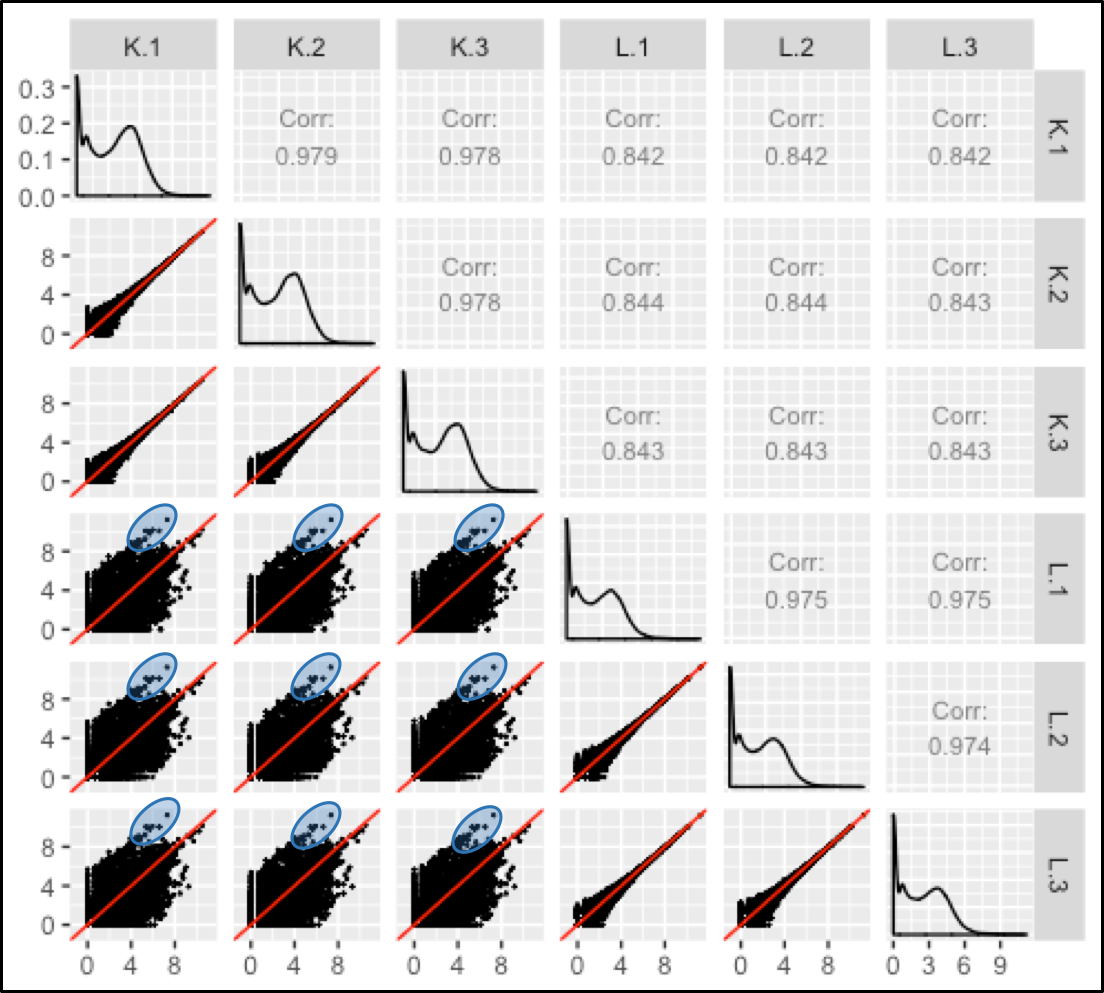
\includegraphics[scale=0.45]{images/lkSM2.png}
\end{figure}
\end{frame}

\begin{frame}{}
\begin{figure}
\centering
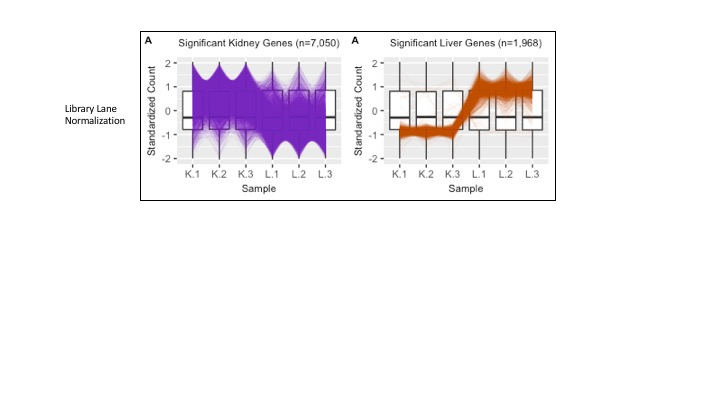
\includegraphics[scale=0.44]{images/lkClusters1.jpg}
\end{figure}
\end{frame}

\begin{frame}[noframenumbering]
\begin{figure}
\centering
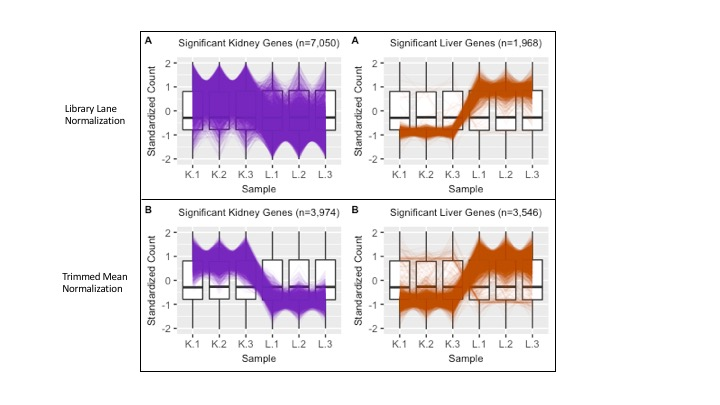
\includegraphics[scale=0.44]{images/lkClusters2.jpg}
\end{figure}
\end{frame}

\begin{frame}[noframenumbering]
\begin{figure}
\centering
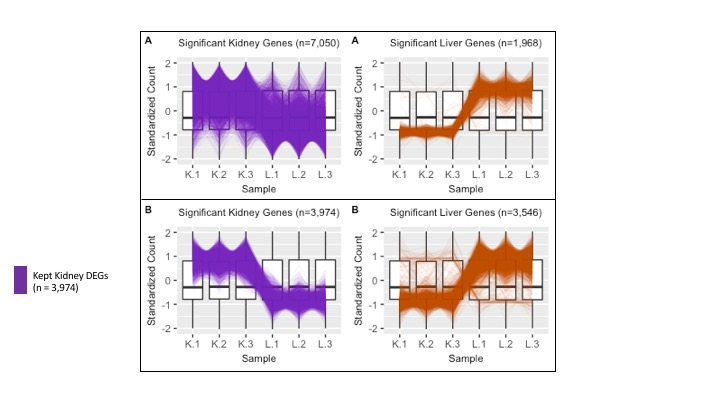
\includegraphics[scale=0.44]{images/lkClusters3.jpg}
\end{figure}
\end{frame}

\begin{frame}[noframenumbering]
\begin{figure}
\centering
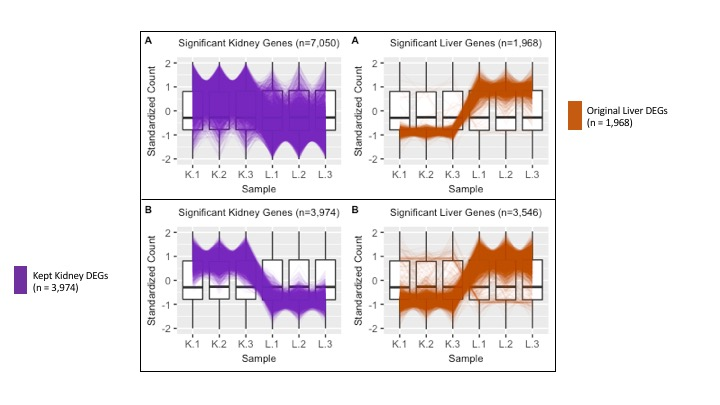
\includegraphics[scale=0.44]{images/lkClusters4.jpg}
\end{figure}
\end{frame}

\begin{frame}[noframenumbering]
\begin{figure}
\centering
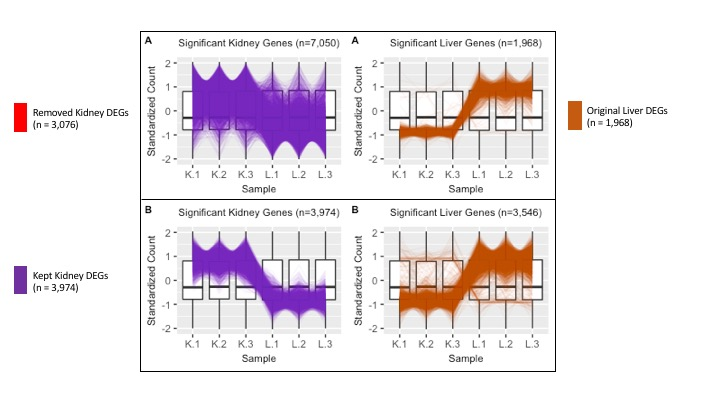
\includegraphics[scale=0.44]{images/lkClusters5.jpg}
\end{figure}
\end{frame}

\begin{frame}[noframenumbering]
\begin{figure}
\centering
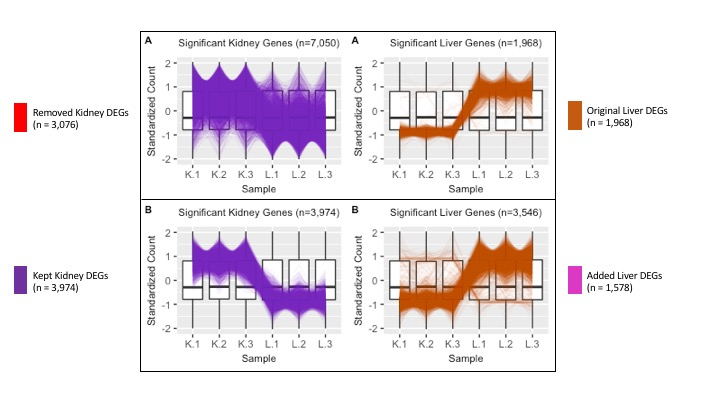
\includegraphics[scale=0.44]{images/lkClusters6.jpg}
\end{figure}
\end{frame}

\begin{frame}{}
\begin{figure}
\centering
\fbox{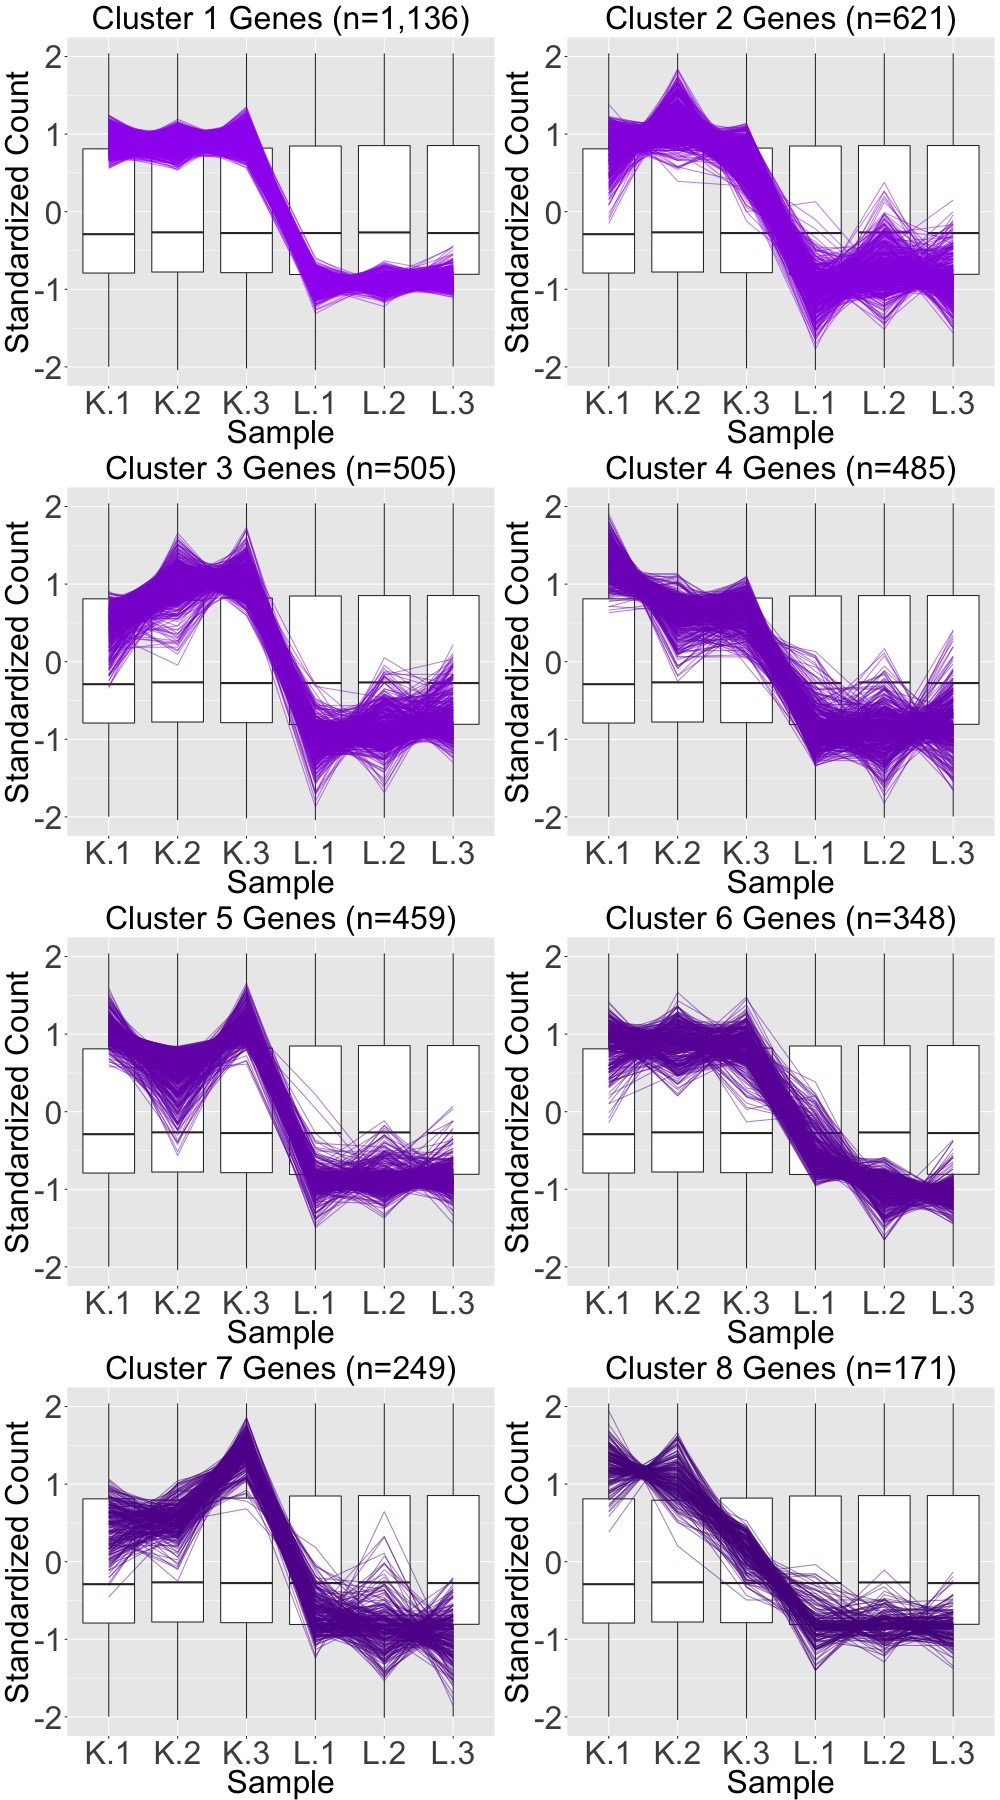
\includegraphics[scale=0.13]{images/lkClustersKeep.jpg}}
\end{figure}
\end{frame}

\begin{frame}{}
\begin{figure}
\centering
\fbox{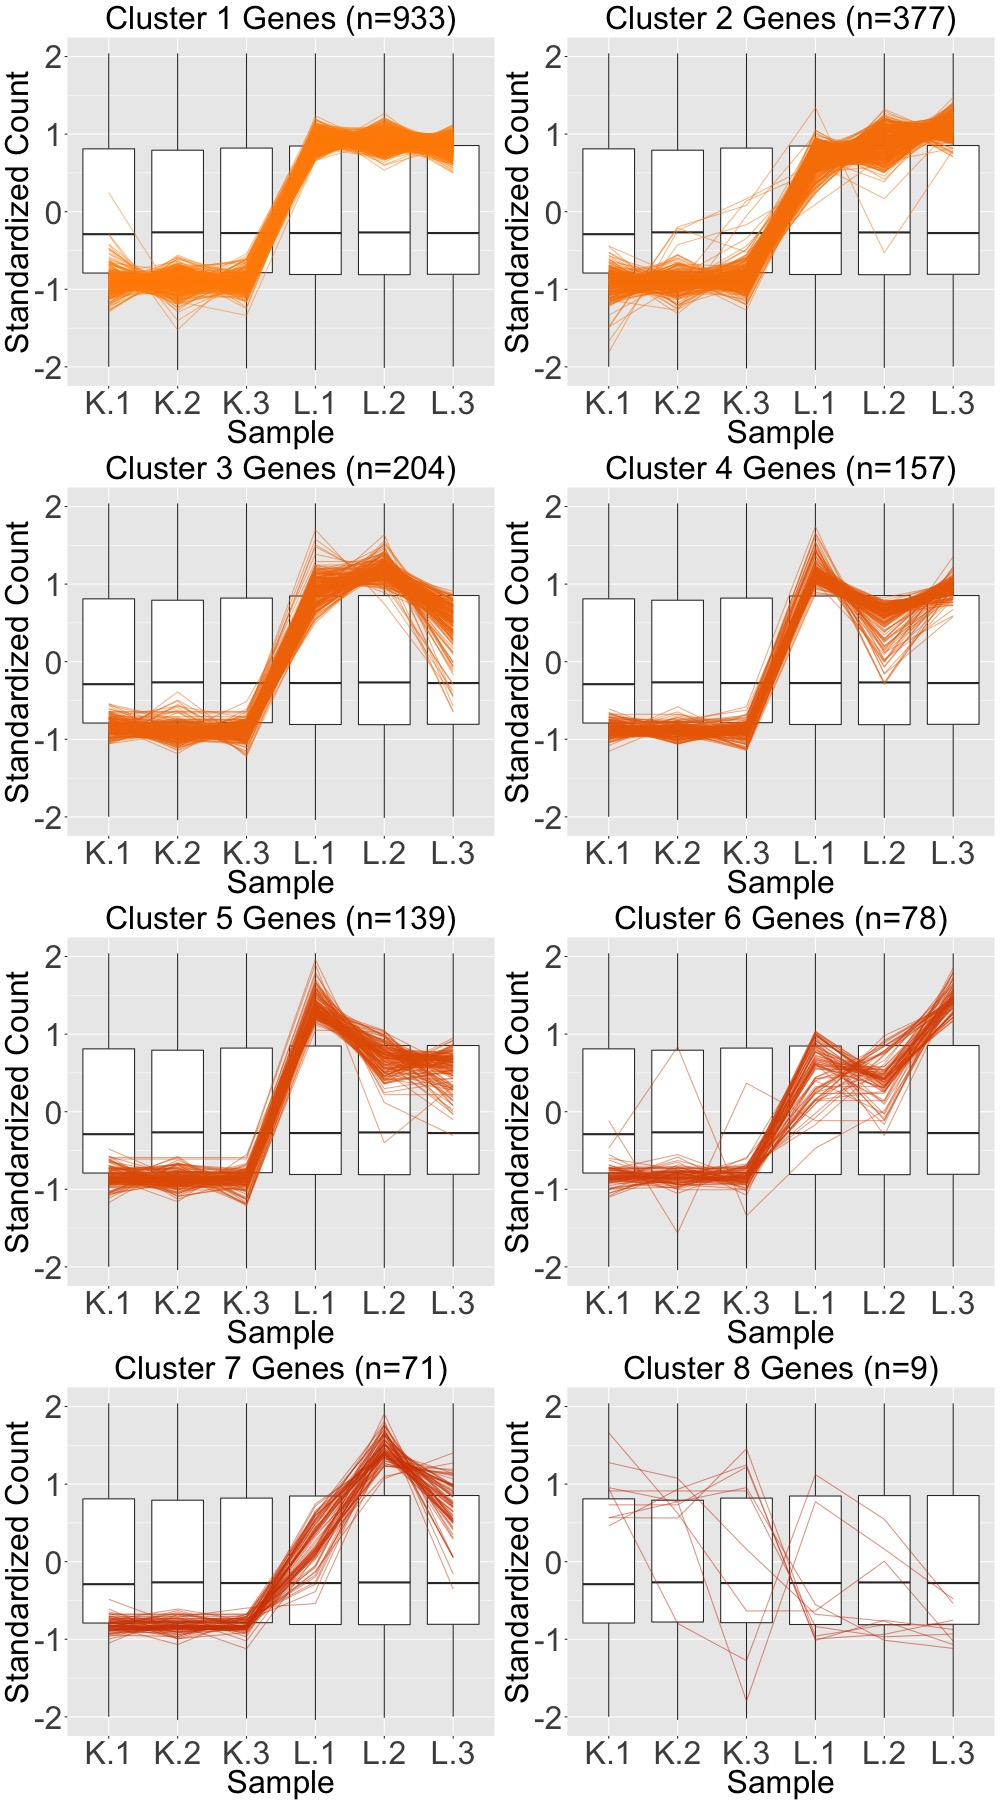
\includegraphics[scale=0.13]{images/lkClustersOrig.jpg}}
\end{figure}
\end{frame}

\begin{frame}{}
\begin{figure}
\centering
\fbox{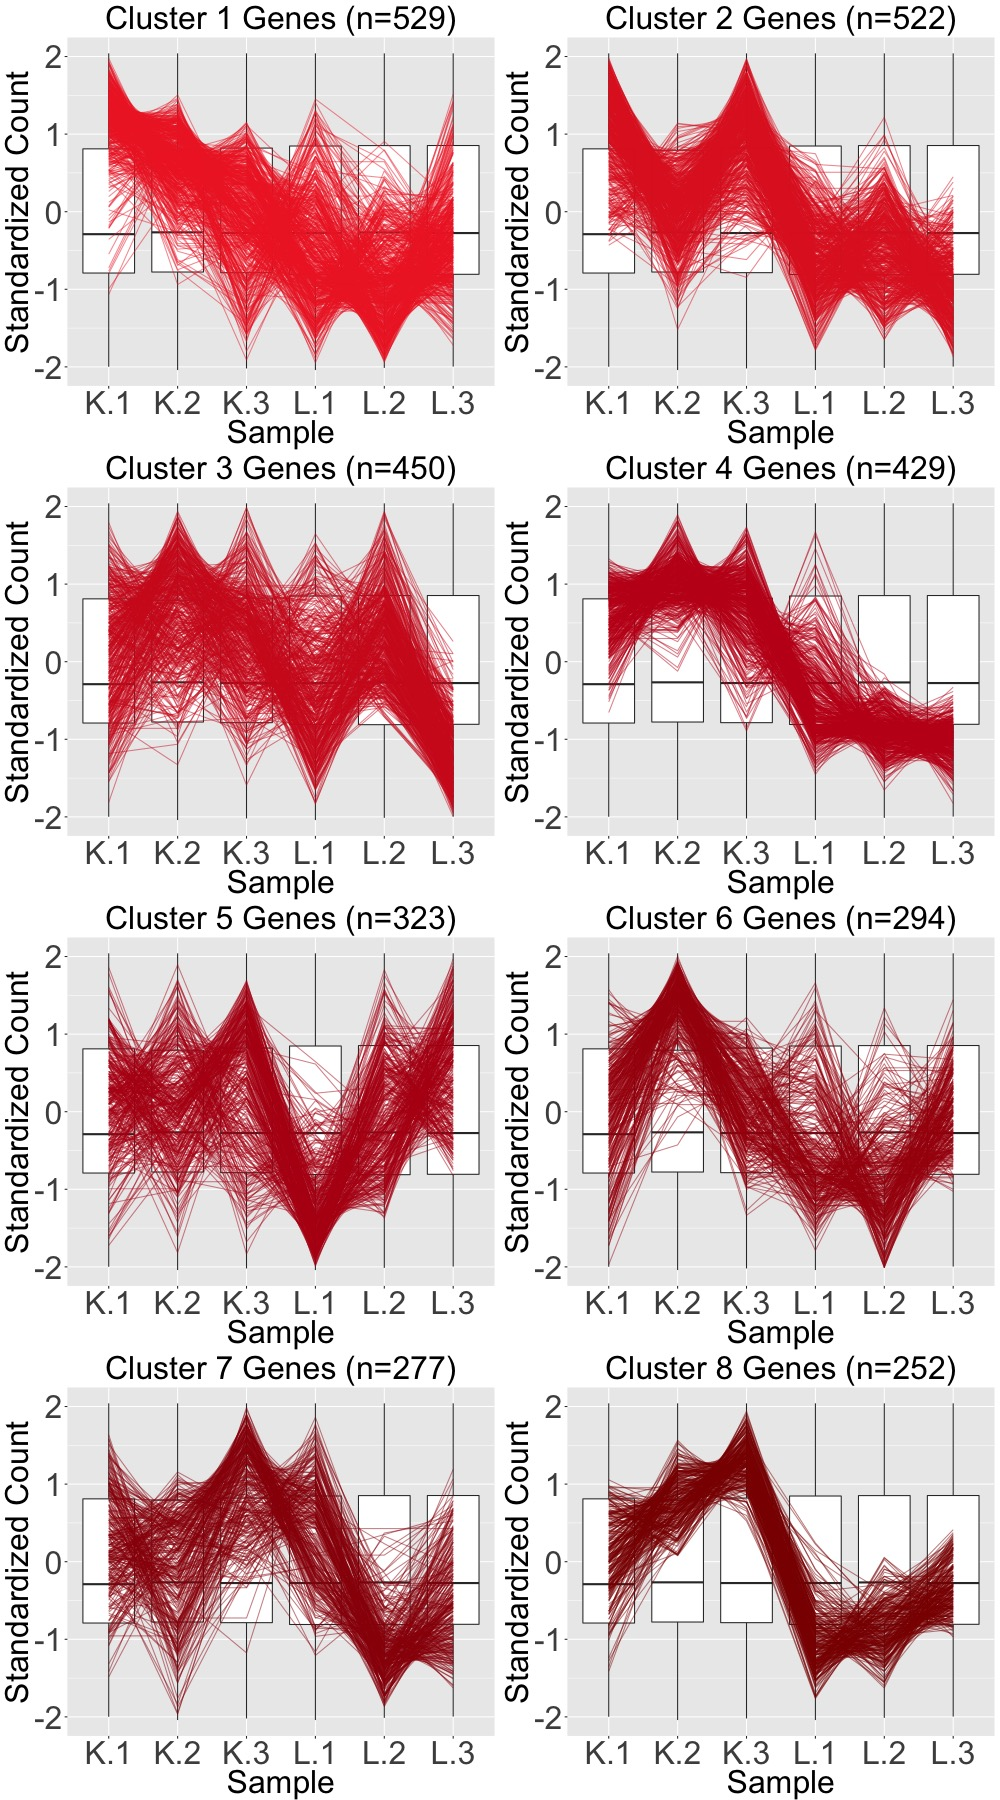
\includegraphics[scale=0.13]{images/lkClustersRemove.jpg}}
\end{figure}
\end{frame}

\begin{frame}{}
\begin{figure}
\centering
\fbox{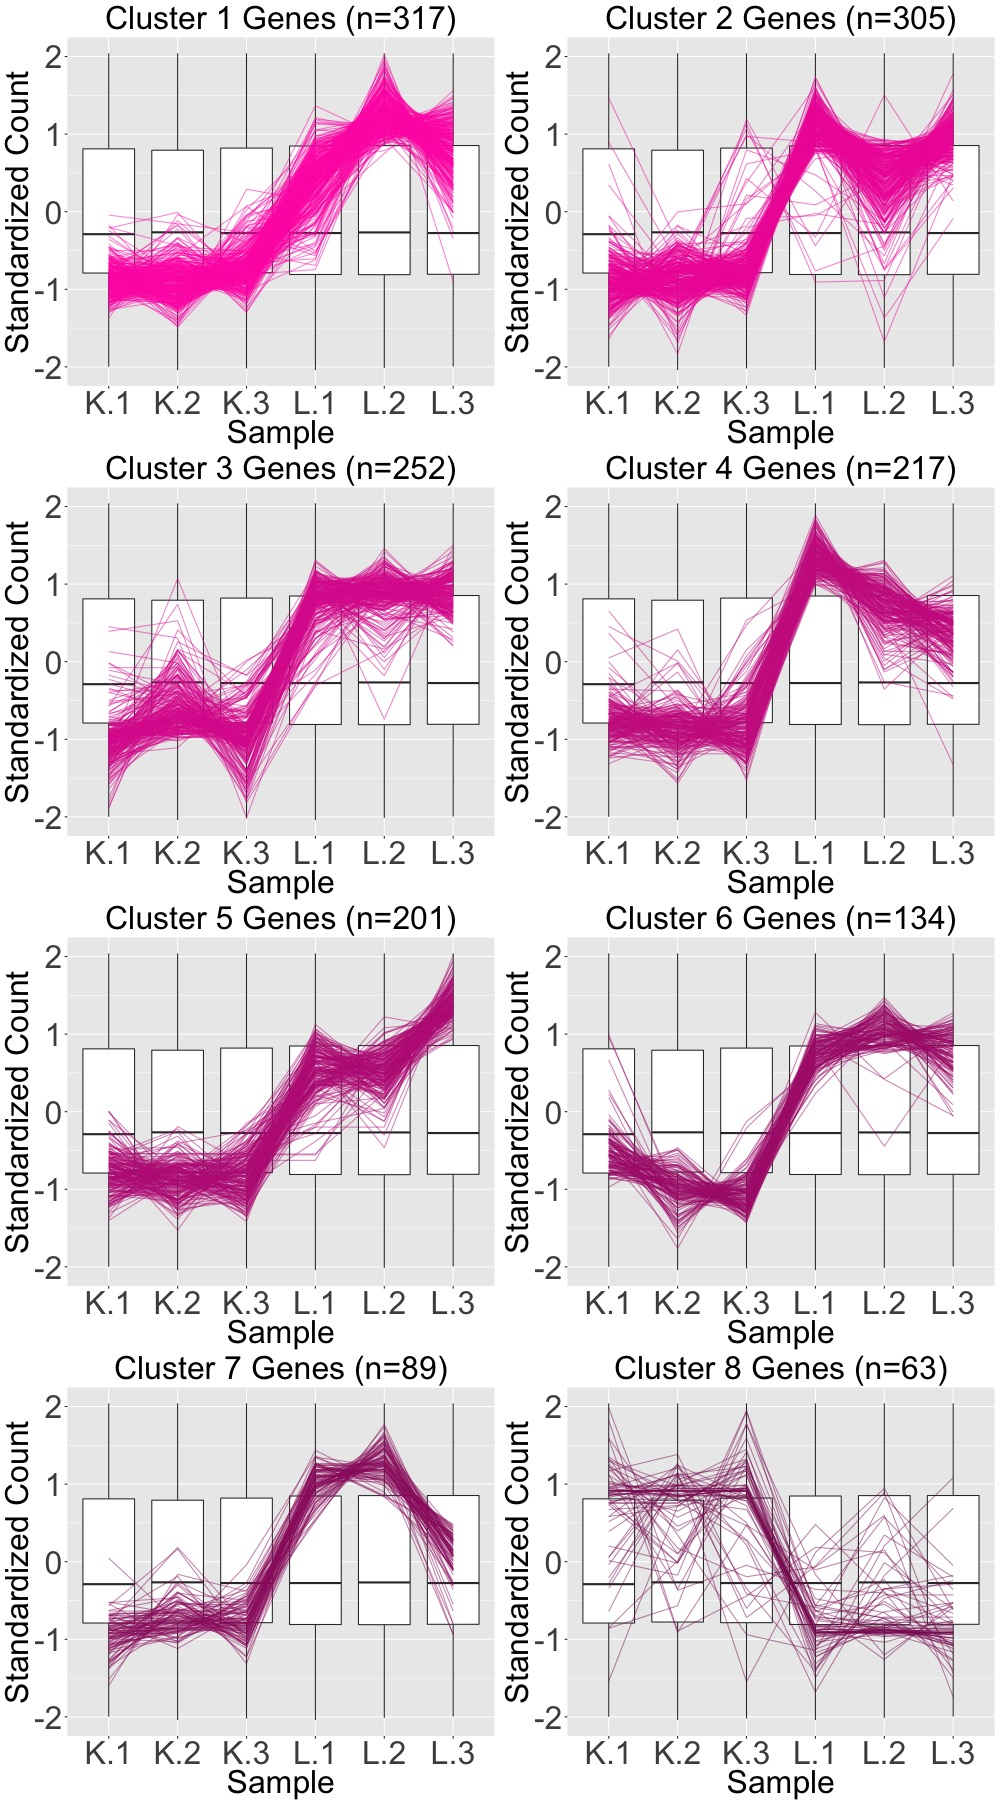
\includegraphics[scale=0.13]{images/lkClustersAdd.jpg}}
\end{figure}
\end{frame}

\begin{frame}{}
\begin{figure}
\centering
\fbox{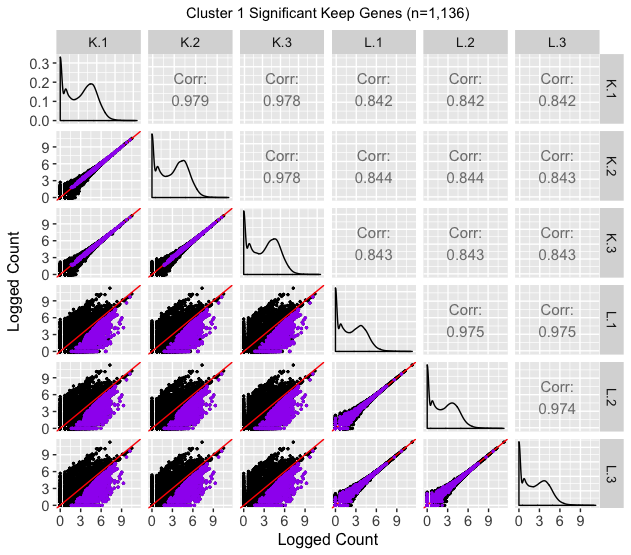
\includegraphics[scale=0.37]{images/lkClustersKeepSM.jpg}}
\end{figure}
\end{frame}

\begin{frame}{}
\begin{figure}
\centering
\fbox{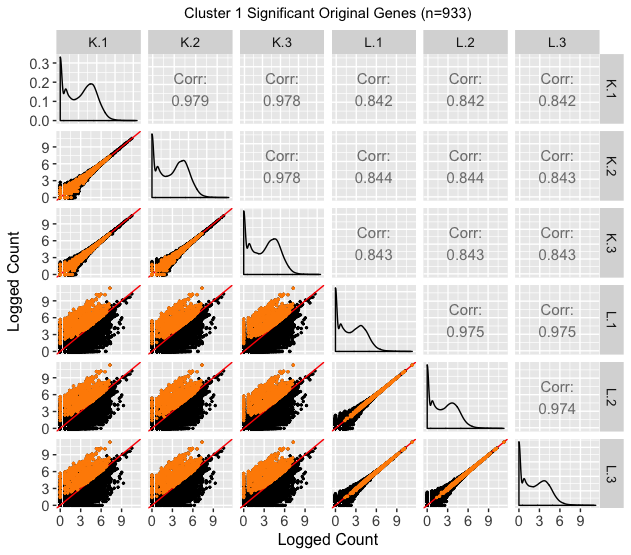
\includegraphics[scale=0.37]{images/lkClustersOrigSM.jpg}}
\end{figure}
\end{frame}

\begin{frame}{}
\begin{figure}
\centering
\fbox{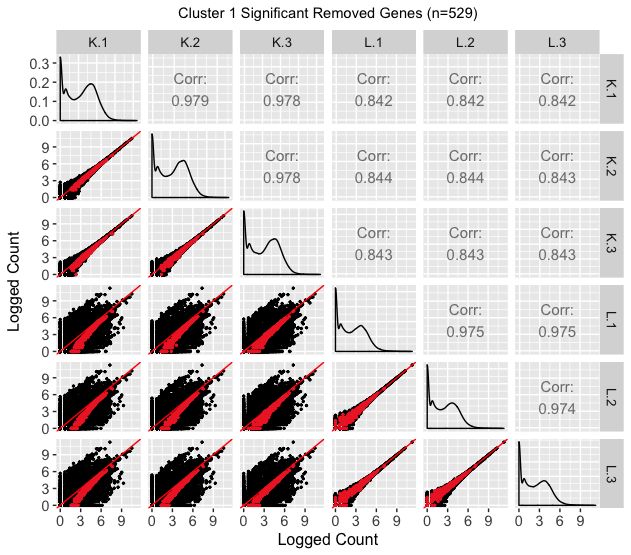
\includegraphics[scale=0.37]{images/lkClustersRemoveSM.jpg}}
\end{figure}
\end{frame}

\begin{frame}{}
\begin{figure}
\centering
\fbox{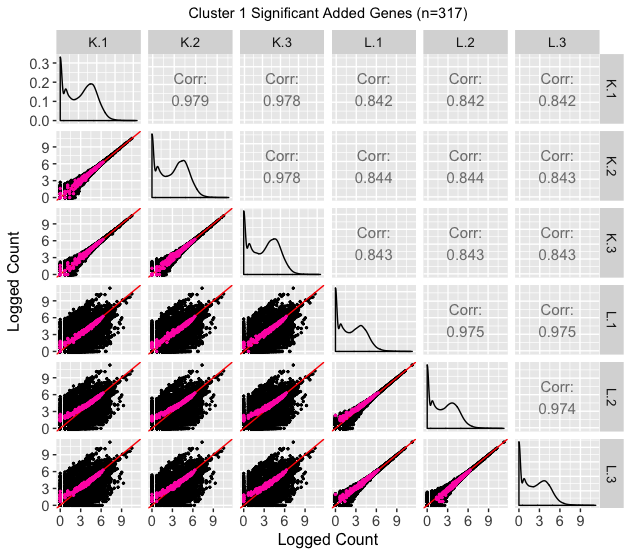
\includegraphics[scale=0.37]{images/lkClustersAddSM.jpg}}
\end{figure}
\end{frame}

\begin{frame}{}
\begin{figure}
\centering
\fbox{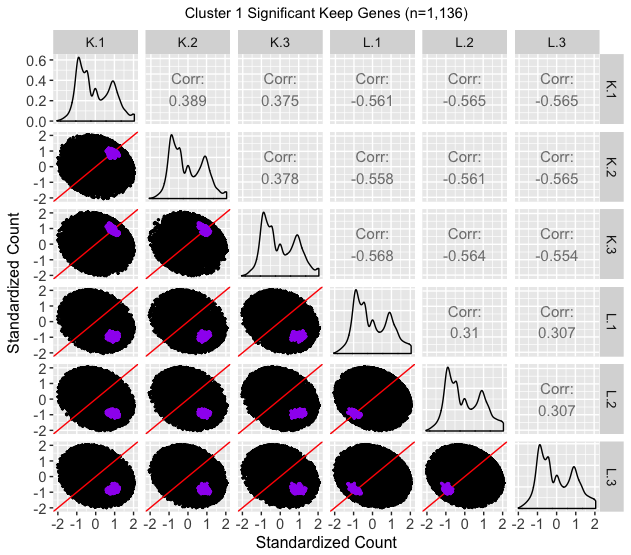
\includegraphics[scale=0.37]{images/lkClustersKeepSM-St.jpg}}
\end{figure}
\end{frame}

\begin{frame}{}
\begin{figure}
\centering
\fbox{\includegraphics[scale=0.37]{images/lkClustersOrigSM-St.jpg}}
\end{figure}
\end{frame}

\begin{frame}{}
\begin{figure}
\centering
\fbox{\includegraphics[scale=0.37]{images/lkClustersRemoveSM-St.jpg}}
\end{figure}
\end{frame}

\begin{frame}{}
\begin{figure}
\centering
\fbox{\includegraphics[scale=0.37]{images/lkClustersAddSM-St.jpg}}
\end{figure}
\end{frame}

\begin{frame}{}
\begin{figure}
\centering
\includegraphics[scale=0.45]{images/litre1.jpg}
\end{figure}
\end{frame}

\begin{frame}[noframenumbering]
\begin{figure}
\centering
\includegraphics[scale=0.45]{images/litre2.jpg}
\end{figure}
\end{frame}

\begin{frame}[noframenumbering]
\begin{figure}
\centering
\includegraphics[scale=0.45]{images/litre3.jpg}
\end{figure}
\end{frame}

\begin{frame}[noframenumbering]
\begin{figure}
\centering
\includegraphics[scale=0.45]{images/litre4.jpg}
\end{figure}
\end{frame}

\begin{frame}[noframenumbering]
\begin{figure}
\centering
\includegraphics[scale=0.45]{images/litre5.jpg}
\end{figure}
\end{frame}

\begin{frame}{}
\begin{figure}
\centering
\fbox{\includegraphics[scale=0.25]{images/litreClusterKeep-St.jpg}}
\end{figure}
\end{frame}

\begin{frame}{}
\begin{figure}
\centering
\fbox{\includegraphics[scale=0.25]{images/litreClusterOrig-St.jpg}}
\end{figure}
\end{frame}

\begin{frame}{}
\begin{figure}
\centering
\fbox{\includegraphics[scale=0.23]{images/litreClusterRemove-St.jpg}}
\end{figure}
\end{frame}

\begin{frame}{}
\begin{figure}
\centering
\fbox{\includegraphics[scale=0.23]{images/litreClusterAdd-St.jpg}}
\end{figure}
\end{frame}


%%%%%%%%%%%%%%%%%%%%%%%%%%%%%%%%% CHAPTER 3 %%%%%%%%%%%%%%%%%%%%%%%%%%%%%
\section{Software to visualize RNA-seq}

\begin{frame}[noframenumbering]
\begin{center}
\fcolorbox{black}{titleColor}{
\begin{minipage}{\textwidth}
\begin{center}
\huge \textbf{Chapter 3:} Software for visualization \\
methods in RNA-seq analysis
\end{center}
\end{minipage}
}
\end{center}
\end{frame}

\begin{frame}
\begin{itemize}
		\item Developing software package \textcolor{ForestGreen}{\textbf{bigPint}}
		\begin{itemize}		  
		  \item BIG multivariate data Plotted INTeractively
		\end{itemize}		
		\item Plan to submit to Bioconductor
		\item Input parameters are popular RNA-seq software output
		\item Methods are built using
		\begin{itemize}
		  \item R
		  \item ggplot2
		  \item plotly
		  \item shiny
		  \item htmlwidgets
		\end{itemize}
	\end{itemize}
\end{frame}

\begin{frame}{}
\begin{figure}
    \centering
    \fbox{\includemedia[width=0.9\textwidth, addresource=images/scatMatPi.mov, deactivate=onclick, flashvars={source=images/scatMatPi.mov}]{\includegraphics{images/scatMatPi.jpg}}{VPlayer.swf}}
\end{figure}
\end{frame}

\begin{frame}{}
\begin{figure}
    \centering
    \fbox{\includemedia[width=0.9\textwidth, addresource=images/volcano.mov, deactivate=onclick, flashvars={source=images/volcano.mov}]{\includegraphics{images/volcano.jpg}}{VPlayer.swf}}
\end{figure}
\end{frame}


% %%%%%%%%%%%%%%%%%%%%%%%%%%%%%%%%% CHAPTER 4 %%%%%%%%%%%%%%%%%%%%%%%%%%%%%
\section{RNA-seq in bees}

\begin{frame}[noframenumbering]
\begin{center}
\fcolorbox{black}{titleColor}{
\begin{minipage}{\textwidth}
\begin{center}
\huge \textbf{Chapter 4:} RNA-seq analysis of diet\\
quality and viral infection in \textit{Apis mellifera}

\end{center}
\end{minipage}
}
\end{center}
\end{frame}

\begin{frame}{Introduction}
\begin{itemize}
	\item Bees have undergone unusually large declines in U.S. and parts of Europe over the past decade
	\item Bees are the leading pollinator of numerous crops so their loss threatens agricultural sustainability 
	\item Bee declines are associated with several factors, likely interactive
	\begin{itemize}
		\item Poor nutrition
	  \item Parasites
	  \item Pesticide use
	  \item Pathogens
	  \item Habitate loss
	\end{itemize}
\end{itemize}
\end{frame}

\begin{frame}{Monofloral diet quality and IAPV}
\begin{itemize}
	\item Bees are confronted with habitat loss and loss of floral diversity and forage
	\begin{itemize}
	  \item Pollen is main source of nutrition
	  \item Mixed-pollen (polyfloral) usually healthier than single-pollen (monofloral)
	  \item Beekeepers rank poor nutrition as one major cause of colony loss
	\end{itemize}
	\item Bees are exposed to viruses more due to spread of ectoparasitic mite
	\begin{itemize}
	  \item Mite feeds on hemolymph and transmits viruses
	  \item Israeli Acute Paralysis Virus (IAPV)
	  \begin{itemize}
	    \item Causes shivering wings, muscle spasms, paralysis, premature death
	    \item High infectious capacity
	    \item Implicated in damaging colony strength and survival    
	  \end{itemize}
	\end{itemize}	
\end{itemize}
\end{frame}

\begin{frame}{Phenotypic findings}
\begin{figure}
\centering
\fbox{\includegraphics[scale=0.47]{images/mortality.png}}
\end{figure}
\end{frame}

\begin{frame}{Current study transcriptomic follow-up}
\begin{itemize}
  \item Aim to understand molecular underpinnings of how good diet buffers against virus-induced mortality
    \begin{itemize}
      \item \textbf{Resistance} (direct and specific effects on immune function)
      \item \textbf{Resilience} (indirect effects on energy availability and vigor)
    \end{itemize}
  \item RNA-seq analysis on four treatment groups
    \begin{itemize}
      \item \textbf{NR}: No viral inoculation and low quality diet (Rockrose)
      \item \textbf{VR}: IAPV viral inoculation and low quality diet (Rockrose)
      \item \textbf{NC}: No viral inoculation and high quality diet (Chestnut)
      \item \textbf{VC}: IAPV viral inoculation and high quality diet (Chestnut)
    \end{itemize}
  \item Compare our results to previous study on bee genomics response to IAPV inoculation
    \begin{itemize}
      \item We used polyandrous colonies (\textbf{25\% genetically identical})
      \item They (Galbraith et al.) used single drone inseminated queen colonies (\textbf{75\% genetically identical})
    \end{itemize}
\end{itemize}
\end{frame}

\begin{frame}{Contrasts}
\begin{figure}
\centering
\includegraphics[scale=0.51]{images/contrasts.jpg}
\end{figure}
\end{frame}

\begin{frame}{Main effect DEG results}
\begin{itemize}
  \item Diet had larger transcriptomic response (n: 1914)
    \begin{itemize}
      \item Chesnut (n: 1033) versus Rockrose (n: 881)
      \item Genes enriched in nutrient signaling (insulin resistance) metabolism and
immune response (Notch signaling and JaK-STAT pathways)
    \end{itemize}
  \item Virus had smaller transcriptomic response (n: 43)
    \begin{itemize}
      \item Virus (n: 38) versus Non-virus (n: 3)
      \item Genes enriched in argonaute-2, transcriptional regulation, and muscle contraction
    \end{itemize}  
\end{itemize}
\end{frame}

\begin{frame}{Other results}
\begin{itemize}
  \item No interaction terms
  \item Resistance candidate genes had functions related to
  \begin{itemize}
    \item Carbohydrate metabolism
    \item Chitin metabolism
    \item Regulation of transcription
    \item Cell adhesion
  \end{itemize}
  \item Resilience candidate genes had functions related to
    \begin{itemize}
    \item Carbohydrate metabolism
    \item Chitin metabolism
    \item Regulation of transcription
    \item Immune response
  \end{itemize}
\end{itemize}
\end{frame}

\begin{frame}{Comparison to Galbraith study}
\begin{figure}
\centering
\fbox{\includegraphics[scale=0.27]{images/C_T_4.jpg}}
\end{figure}
\end{frame}

\begin{frame}{Comparison to Galbraith study}
\begin{figure}
\centering
\fbox{\includegraphics[scale=0.36]{images/N_V_4.png}}
\end{figure}
\end{frame}

\begin{frame}{Comparison to Galbraith study}
\begin{figure}
\centering
\fbox{\includegraphics[scale=0.3]{images/litreClusterRutter.png}}
\end{figure}
\end{frame}

\begin{frame}{Comparison to Galbraith study}
\begin{figure}
\centering
\fbox{\includegraphics[scale=0.3]{images/litreCluster2.png}}
\end{figure}
\end{frame}

\begin{frame}{Comparison to Galbraith study}
\begin{figure}
\centering
\includegraphics[scale=0.45]{images/GRVenn.png}
\end{figure}
\end{frame}

% %%%%%%%%%%%%%%%%%%%%%%%%%%%%%%%%% CONCLUSIONS %%%%%%%%%%%%%%%%%%%%%%%%%%%%%

\begin{frame}{Conclusions}
\begin{itemize}
  \item RNA-seq should be approached with both models and visualization
    \begin{itemize}
      \item Future direction: Collect more examples
    \end{itemize}
  \item RNA-seq visualization tools will be available on bigPint
    \begin{itemize}
      \item Future direction: Increase interactivity speed
      \item Future direction: Create helpful user manual
    \end{itemize}
\end{itemize}
\end{frame}

\begin{frame}[noframenumbering]{Acknowledgements}
\begin{itemize}
  \item POS Committee for support with thesis development
  \begin{itemize}
    \item Amy Toth (Major Professor)
    \item Dianne Cook (Major Professor)
    \item Heike Hofmann
    \item Daniel Nettleton
    \item James Reecy
  \end{itemize}
  \item Susan VanderPlas for developing the beginning of the ggenealogy project 
  \item Adam Dolezal for completing the wet-lab component of the honeybee study
  \item Roxane Legaie for serving as a summer mentor for bigPint software development
  \item Adrienne Moran Lauter and Michelle Graham for sharing iron-metabolism soybean data
\end{itemize}
\end{frame}

\begin{frame}[noframenumbering]{GitHub Resource}

  \centering \huge{https://github.com/lrutter/bigPint}

\end{frame}

\end{document}
